
\documentclass[conference]{IEEEtran}
\usepackage[english]{babel}
\usepackage[utf8]{inputenc}
\usepackage{graphicx}
\usepackage[colorinlistoftodos]{todonotes}
\usepackage{blindtext, graphicx}
\usepackage{hyperref}
\usepackage{caption}
\usepackage{float}
\usepackage{balance}
\usepackage{listings}
\renewcommand{\thesubsection}{\arabic{subsection}}
\usepackage{amsmath}


\ifCLASSINFOpdf
\else
\fi

\begin{document}

\pagestyle{plain}

\title{When making up data is a good idea: On the advantages of partially synthetic training sets for software analytics}

\author{\IEEEauthorblockN{Amritanshu Agrawal}
\IEEEauthorblockA{Department of Computer Science\\
North Carolina State University\\
Raleigh, NC, USA\\
Email: aagrawa8@ncsu.edu}
\and
\IEEEauthorblockN{Raghavendra Prasad Potluri}
\IEEEauthorblockA{Department of Computer Science\\
North Carolina State University\\
Raleigh, NC, USA\\
Email: rpotlur@ncsu.edu}}

\maketitle

\begin{abstract}
The accurate prediction of where faults are likely to occur in code can help direct test effort, reduce costs and improve the quality of software. One of the approaches to tackle the problem, is based on relying on code metrics especially CK metrics. The aim of the project was to reproduce a package showing comparative study of 6 learners for defect prediction using CK metrics. We successfully made a python pip package and also found an astonishing result. Using SMOTE brought out a clear winner of which learner to use. Other users will now be able to use this package and refute our results as well as get future results in no time. There are still various improvements that can be done which we will be publishing in our next revised package.
\end{abstract}

\begin{IEEEkeywords}
Defects prediction, code metrics, classification.
\end{IEEEkeywords}

\IEEEpeerreviewmaketitle

\section{Introduction}
Software defect prediction has been an important research topic in the software engineering field for more than 30 years. It has generated widespread interest for a
considerable period of time. The driving scenario is resource
allocation: Time and manpower being finite resources, it
makes sense to assign personnel and/or resources to areas of
a software system with a higher probable quantity of defects. Current defect prediction work focuses on (i) estimating the number of defects remaining in software systems, (ii) discovering defect associations, and (iii) classifying the defect-proneness of software components, typically into two classes defect-prone and not defect-prone. 

There have been vast amount of studies done to find the best defect prediction performing model. But literature suggests, that no single prediction technique dominates and making sense of the many prediction results is hampered by the use of different data sets, data pre-processing, validation schemes and performance
statistics. We highly agree to this given so many variations available in the data and there are so many classification techniques available like Statistical, Clustering, Rule-Based, Neural Networks, Nearest Neighbour, Support Vector Machines, Decision trees, ensemble methods, to name a few.

This project deals with the third type of problem for code metrics which is classifying the defect-proneness of software components, typically into two classes defective and not defective. Ghotra et al.~\cite{ghotra2015revisiting} did a comparative study on various learners for defect prediction. They found out that mainly 6 learners have been performing well namely Naive Bayes, Logistic regression, Support Vector Machines, Nearest Neighbor, decision tree and Random forest. Our project considered Ghotra et al. results as the baseline results.

For the reproduction package we generalised our datasets to be comprised of CK metrics~\cite{chidamber1994metrics}. The CK metrics aim at measuring whether a piece of code follows OO principles. It contains a check of these OO design attributes:
\begin{itemize}
 \item {\textbf{Weighted Methods for Class (WMC)}}
 The sum of the complexities of each method in a class. If all the method complexities are considered equal and have the value of 1 (as proposed in the chidamber94), then WMC equals the number of methods in a class.
 \item {\textbf{Depth of Inheritance Tree (DIT)}}
 Number of classes that a particular class inherits from.
 \item {\textbf{Number of Children (NOC)}}
 The count of immediate subclasses of a class.
 \item {\textbf{Response for Class (RFC)}}
 The number of elements in the response set of a class. The response set of a class (as defined in chidamber94) is the number of methods that can potentially be executed in response to a message received by an object of that class.
 \item {\textbf{Lack of Cohesion of Methods (LCOM)}}
 For a class C, LCOM is the number of method pairs that have no common references to instance variables minus the number of method pairs that share references to instance variables.
 \item {\textbf{Coupling Between Objects (CBO)}}
 For a class C, CBO is the number of classes that are coupled to (i.e. call a function or access a variable of) C.
\end{itemize}

We created a Pip Package generalised to run any CK metrics based dataset and compare results against 6 learners. Since the classes are imbalanced (less defective class about 15 percent), we used SMOTE~\cite{chawla2002smote} (only on Training Data) which is a synthetic minority over-sampling technique.

The remainder of this report is organized as follows. Section \ref{review} gives a brief related work on defect prediction. Since we found an astonishing results on smote, section \ref{smote} tells about SMOTE. Experimental setup is provided in section \ref{experiment}. Then results are discussed in Section \ref{results}. Final conclusion is being discussed in section \ref{conclusion}. And section \ref{future} talks about future work.

\section{Related Work}
\label{review}

There are works on defect prediction which employs statistical approaches, capture-recapture (CR) models,
and detection profile methods (DPM)~\cite{song2011general}. The second type of work borrows association rule mining
algorithms from the data mining community to reveal software defect associations~\cite{song2006software}. A variety of approaches have been proposed to tackle the third type of problem, relying on diverse information, such as code metrics~\cite{nagappan2006mining,d2010extensive, hall2012systematic,radjenovic2013software,shepperd2014researcher} (lines of code, complexity), process metrics~\cite{hassan2009predicting} (number of changes, recent activity) or previous defects~\cite{kim2007predicting}.

Some other research~\cite{bird2009putting} indicate that it is possible to predict which components are likely locations of
defect occurrence using a component’s development history,
and dependency structure. Two key properties of software components
in large systems are dependency relationships (which components
depend on or are dependent on by others), and development
history (who made changes to the components and
how many times). Thus we can link software components
to other components a) in terms of their dependencies, and
also b) in terms of the developers that they have in common. Prediction models based on the topological properties
of components within them have proven to be quite
accurate~\cite{zimmermann2008predicting}.

Result by Tantithamthavorn et al.~\cite{tantithamthavorn2016automated} also suggested that every dataset comes with different attributes. And also classification techniques often have configurable parameters
that control characteristics of these classifiers that they produce. Now time has come to even think about hyperparameter optimization of these techniques and come up with an automated process~\cite{fu2016tuning,agrawal2016wrong} to tune these parameters for every dataset.

And lastly we found a paper from Ghotra et al.~\cite{ghotra2015revisiting} on "Revisiting the impact of classification techniques on the performance of defect prediction models". To  compare  the  performance  of  defect prediction  models,  they  used  the  Area  Under  the receiver operating characteristic Curve (AUC), which plots  the  false  positive  rate  against  the  true  positive rate. They ran the Scott-Knott test to group classification techniques into statistically distinct ranks

\section{Case Study of SMOTE in Defect Prediction}
\label{smote}
There have been various oversampling and undersampling techniques available. And SMOTE~\cite{chawla2002smote} has become increasingly popular in recent times. To find out the effects of smote in Software defect prediction, we found out few papers. Some researchers~\cite{gray2009using,wang2013using} studied various undersampling and oversampling technique and compared the results with Naive Bayes and random forest. Some found out that AdaBoost.NC had a better performance than the rest while others are planning to use SMOTE. Overall oversampling and undersampling of data has been useful.

Pelayo et al.~\cite{pelayo2007applying} studied the effects of percentage of oversampling and undersampling done. They found out that different percentage of each helps improve the accuracies of decision tree learner for defect prediction using CK metrics.

\section{Experimental Setup}
\label{experiment}

\subsection{\textbf{Data}}
 We used the data sets available in promise repository\footnote{http://openscience.us/repo/defect/ck/}. Totally 14 data sets are used. These datasets have been collected from the work done by Jureczko et al.~\cite{jureczko2010towards}. Namely these datasets are:
 \begin{itemize}
 \item ANT
 \item ARC
 \item CAMEL
 \item IVY
 \item JEDIT
 \item LOG4J
 \item POI
 \item REDAKTOR
 \item SYNAPSE
 \item TOMCAT
 \item VELOCITY
 \item XALAN
 \item XERCE
\end{itemize}

\subsection{\textbf{Preprocessing}}
CK metrics comprises mostly of numerals. But to generalize the package we added pre-processing component. We ignore any string columns in the data. We assume the last column in the data sets is the class label. Originally, the target class contains number of defects. We converted them into binary, i.e if target class has defect then it represents 1 otherwise its 0. The package assumes user has preprocessed the data before passing it to the learners. 

\subsection{\textbf{Classifiers}}
We used six classifiers which are mentioned in the baseline paper~\cite{ghotra2015revisiting}. Beside every learner we wrote some important parameter which are hardcoded as suggested by Ghotra et al.
\begin{itemize}
 \item \textbf{Support Vector Machine (Linear Kernel)}
 In machine learning, support vector machines (SVMs, also support vector networks) are supervised learning models with associated learning algorithms that analyze data used for classification and regression analysis. Given a set of training examples, each marked as belonging to one or the other of two categories, an SVM training algorithm builds a model that assigns new examples to one category or the other, making it a non-probabilistic binary linear classifier.
 \item \textbf{Logistic Regression}
 In statistics, linear regression is an approach for modeling the relationship between a scalar dependent variable y and one or more explanatory variables (or independent variables) denoted X.
 \item \textbf{Naive Bayes}
 In machine learning, naive Bayes classifiers are a family of simple probabilistic classifiers based on applying Bayes theorem with strong (naive) independence assumptions between the features.
 \item \textbf{K Nearest Neighbors (K=8)}
 In pattern recognition, the k-Nearest Neighbors algorithm (or k-NN for short) is a non-parametric method used for classification and regression. In both cases, the input consists of the k closest training examples in the feature space.
 \item \textbf{Decision Trees (CART, Split Criteria=Entropy)}
 A decision tree is a decision support tool that uses a tree-like graph or model of decisions and their possible consequences, including chance event outcomes, resource costs, and utility. It is one way to display an algorithm.
 \item \textbf{Random Forest (Split Criteria=Entropy)}
 Random forests or random decision forests are an ensemble learning method for classification, regression and other tasks, that operate by constructing a multitude of decision trees at training time and outputting the class that is the mode of the classes (classification) or mean prediction (regression) of the individual trees. 
\end{itemize}

We are using K=8 for K Nearest Neighbours because it was proposed to perform better. Also for Decision trees and Random Forest we are using Entropy as split criteria. Scikit-Learn~\cite{pedregosa2011scikit} provides this feature of selecting the split criteria. Since the classes are highly imbalanced we want training and testing set to have same proportions of both the classes. That's why we used stratified 5- Fold Cross-validation as default.

\subsection{\textbf{Package}}

We implemented the package in Python 2.7 but added support for Python 3.x as well. Our package depends on scikit-learn and NLTK. It has been written in pep8 standards to ensure it can be deployed in pip. Users can import Learner module, which requires file name as mandatory parameter, folds and splits as optional parameters. The default values of folds and splits are 5, and 5 respectively. The smoting can be turned on or off by passing smoting flag to the learner. We are using "ball tree" nearest neighbor algorithm for smoting. The run method accepts a list of learners to be used. 

\begin{lstlisting}
Sample Execution:
    import Learner
    learner = Learner("./data/ant.csv")
    learner.run()
    learner.stats()
\end{lstlisting}

The execution procedure is 
\begin{itemize}
\item Csv file input is parsed. Converting integers to float.
\item The data is now shuffled and dropped into bins using StratifiedKFold.
\item The unbalanced class is smoted, depends on the user choice.
\item Data is passed to each learner and its predicted value for target class is captured.
\item A stats file (Scott-Knott) is used to calculate the measures using the predicted target class.
\item The stats are aggregated in result object and displayed upon execution of all learners.
\end{itemize}

There are certain helper functions for user to just calculate one or more of the measures, recall, f1 score, accuracy, precision and false alarm. A helper function to display available learners is also implemented.

\subsection{\textbf{Evaluation Measures}}

Since, this is a multi-class classification problem, we represent the predictions using a confusion matrix where a `positive' output is the class under study and a `negative' output is the non defective class. The confusion matrix is shown in figure \ref{fig:cmatrix}.

\begin{figure}[!htpb]
    \centering
    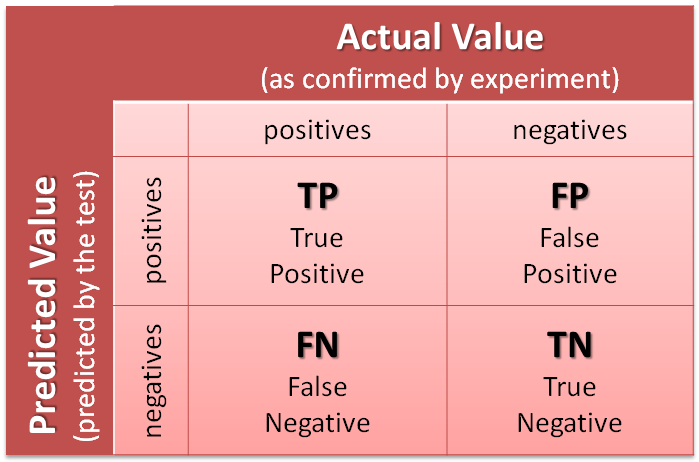
\includegraphics[scale=0.35]{cmatrix.png}
    \caption{Confusion Matrix}

    \label{fig:cmatrix}
\end{figure}

We define the measures as
\begin{itemize}
\item \textbf{Recall}  is the fraction of relevant instances that are retrieved.
\[Recall(rec) = \dfrac{TP}{TP + FN}\]
\item \textbf{Precision} is the fraction of retrieved instances that are relevant.
\[Precision(prec) = \dfrac{TP}{TP + FP}\]
\item \textbf{F1 Score} A measure that combines precision and recall which is the harmonic mean of precision and recall.
\[F1 = \dfrac{2*prec*rec}{prec + rec}\]
\item \textbf{Accuracy} is a weighted arithmetic mean of Precision and Inverse Precision (weighted by Bias) as well as a weighted arithmetic mean of Recall and Inverse Recall.
\[Accuracy = \dfrac{TP + TN}{TP + FP + FN + TN}\]
\item \textbf{False Alarm} is the ratio of false positive to predicted negative total.
\[False alarm(pf) = \dfrac{FP}{FP + TN}\]
\end{itemize}


\begin{figure*}[!htbp]
    \centering
    \begin{minipage}[b]{0.49\linewidth}
        \begin{center}
        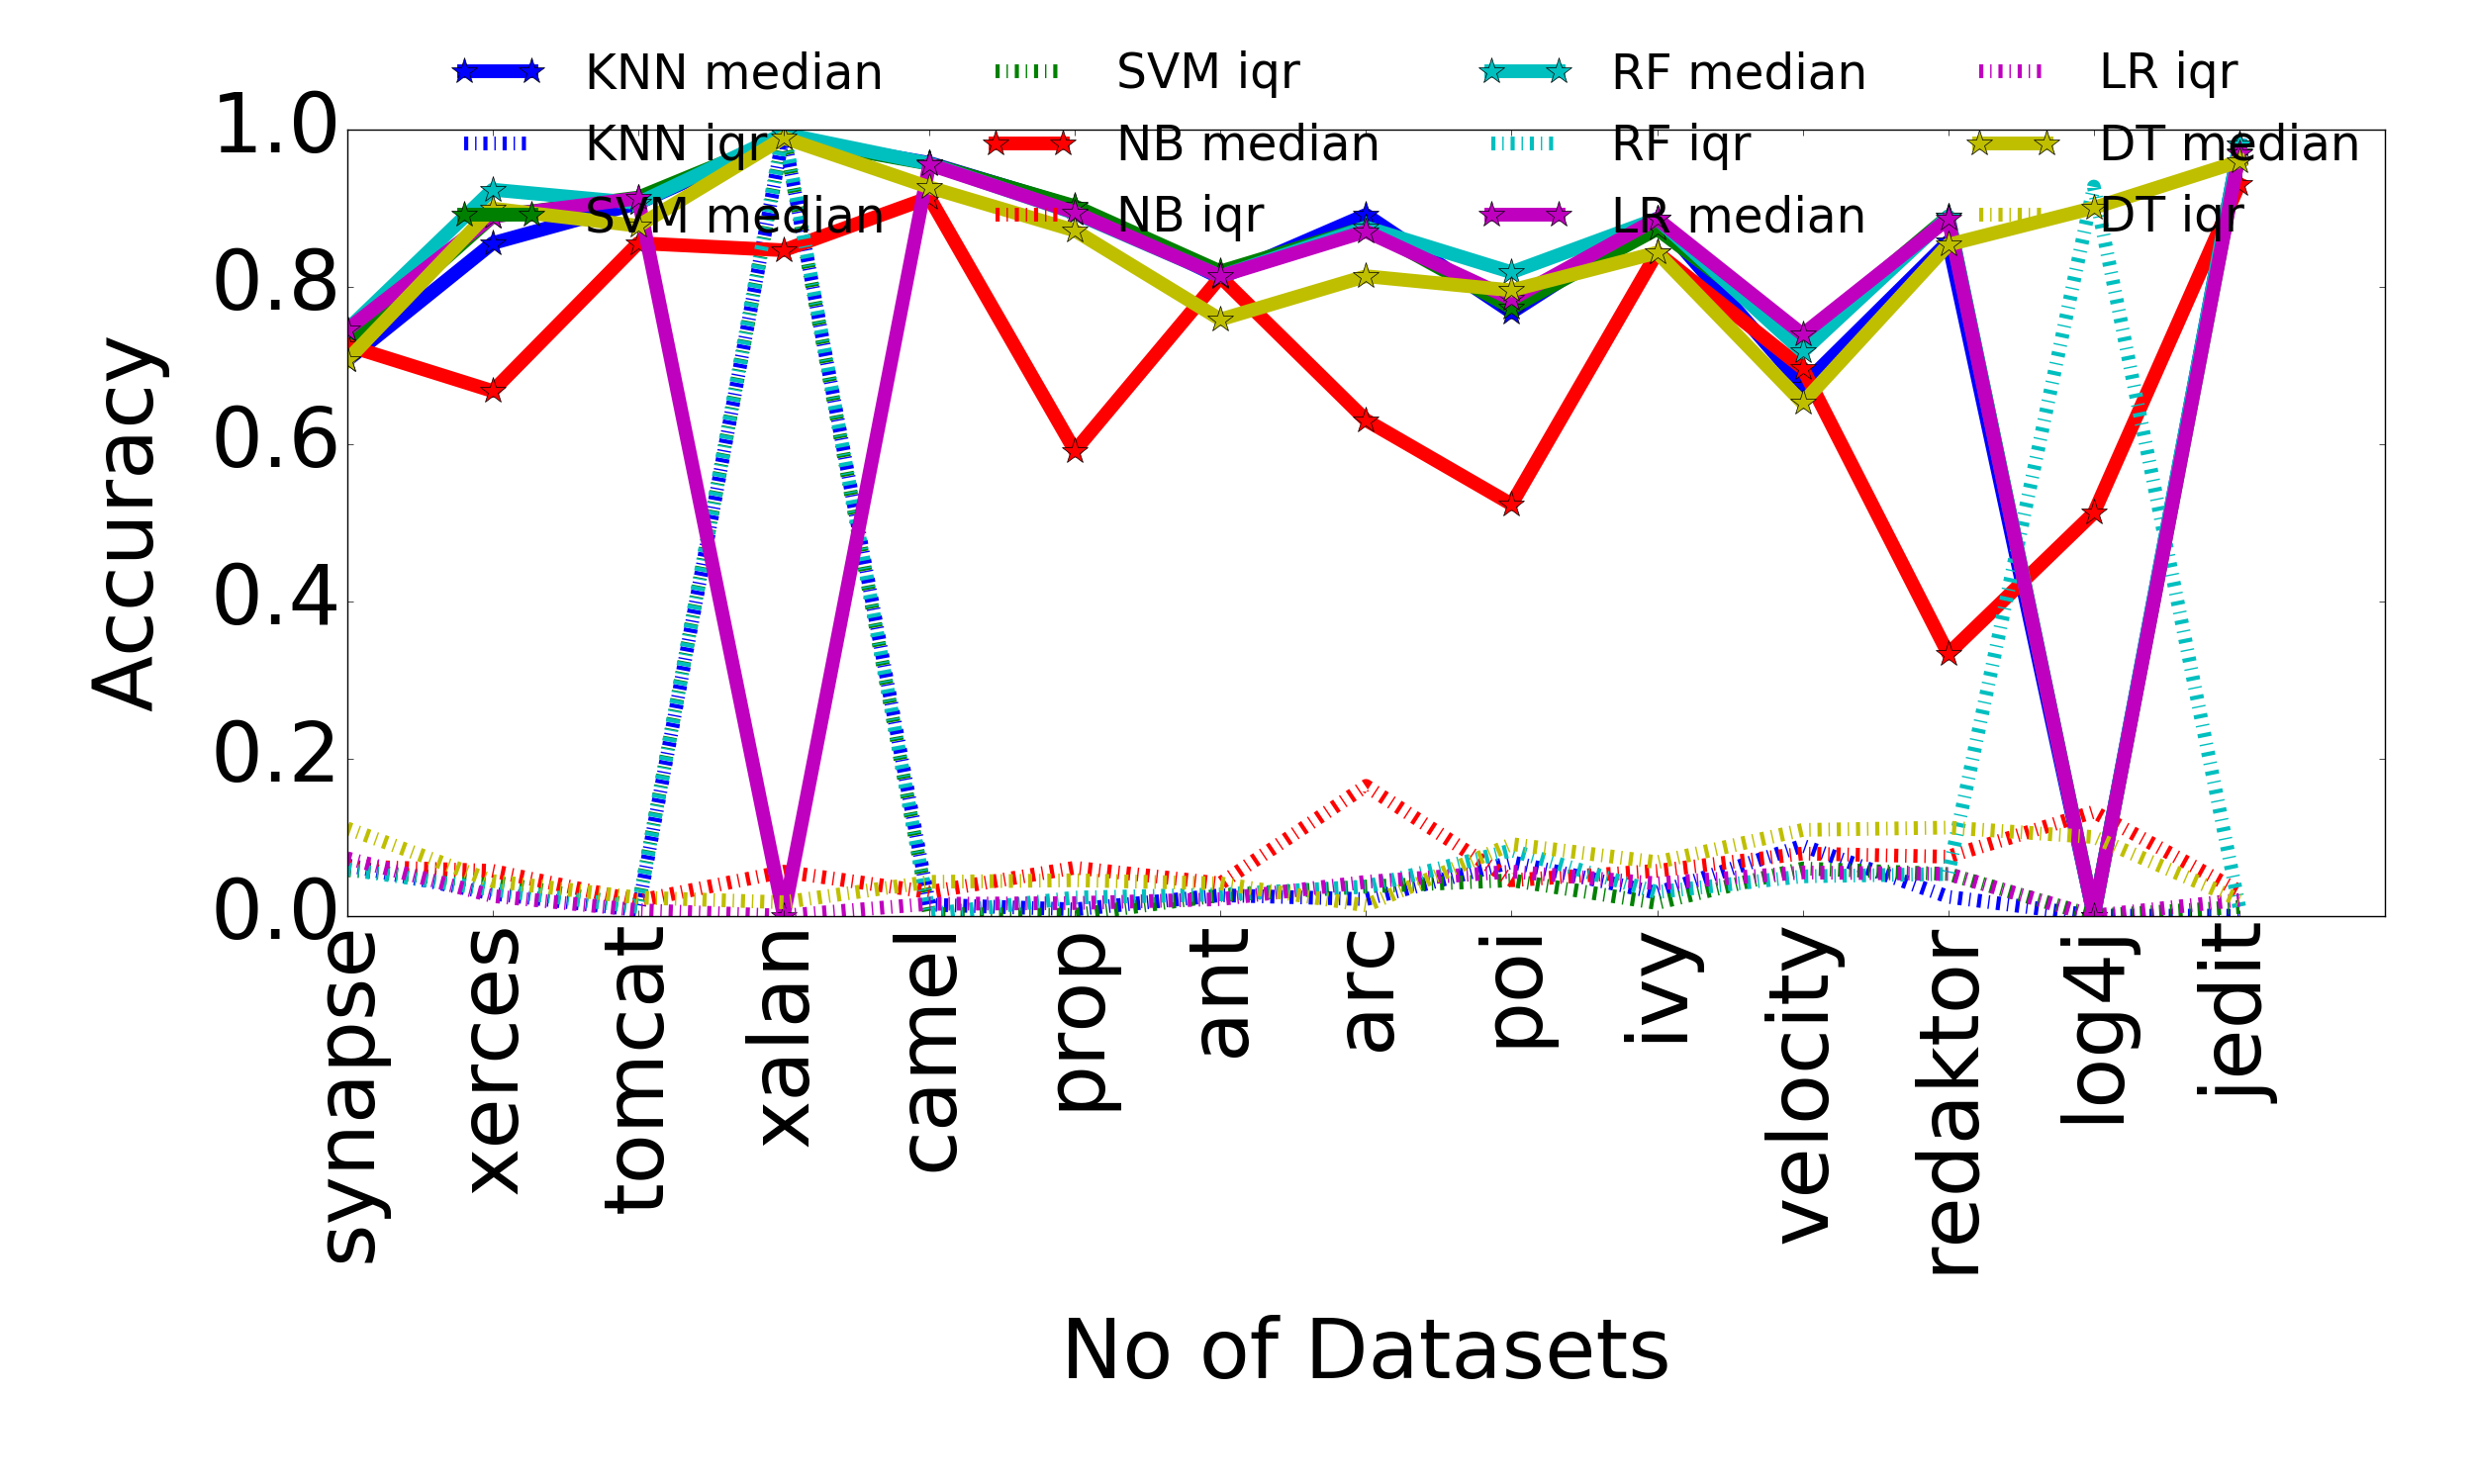
\includegraphics[width=\linewidth]{Accuracy_nosmote.png}
  {\bf Figure~\ref{fig:nosmote}a:} Accuracy Without smote.
  \end{center}
    \end{minipage}%
    \begin{minipage}[b]{0.49\linewidth}
        \begin{center}
        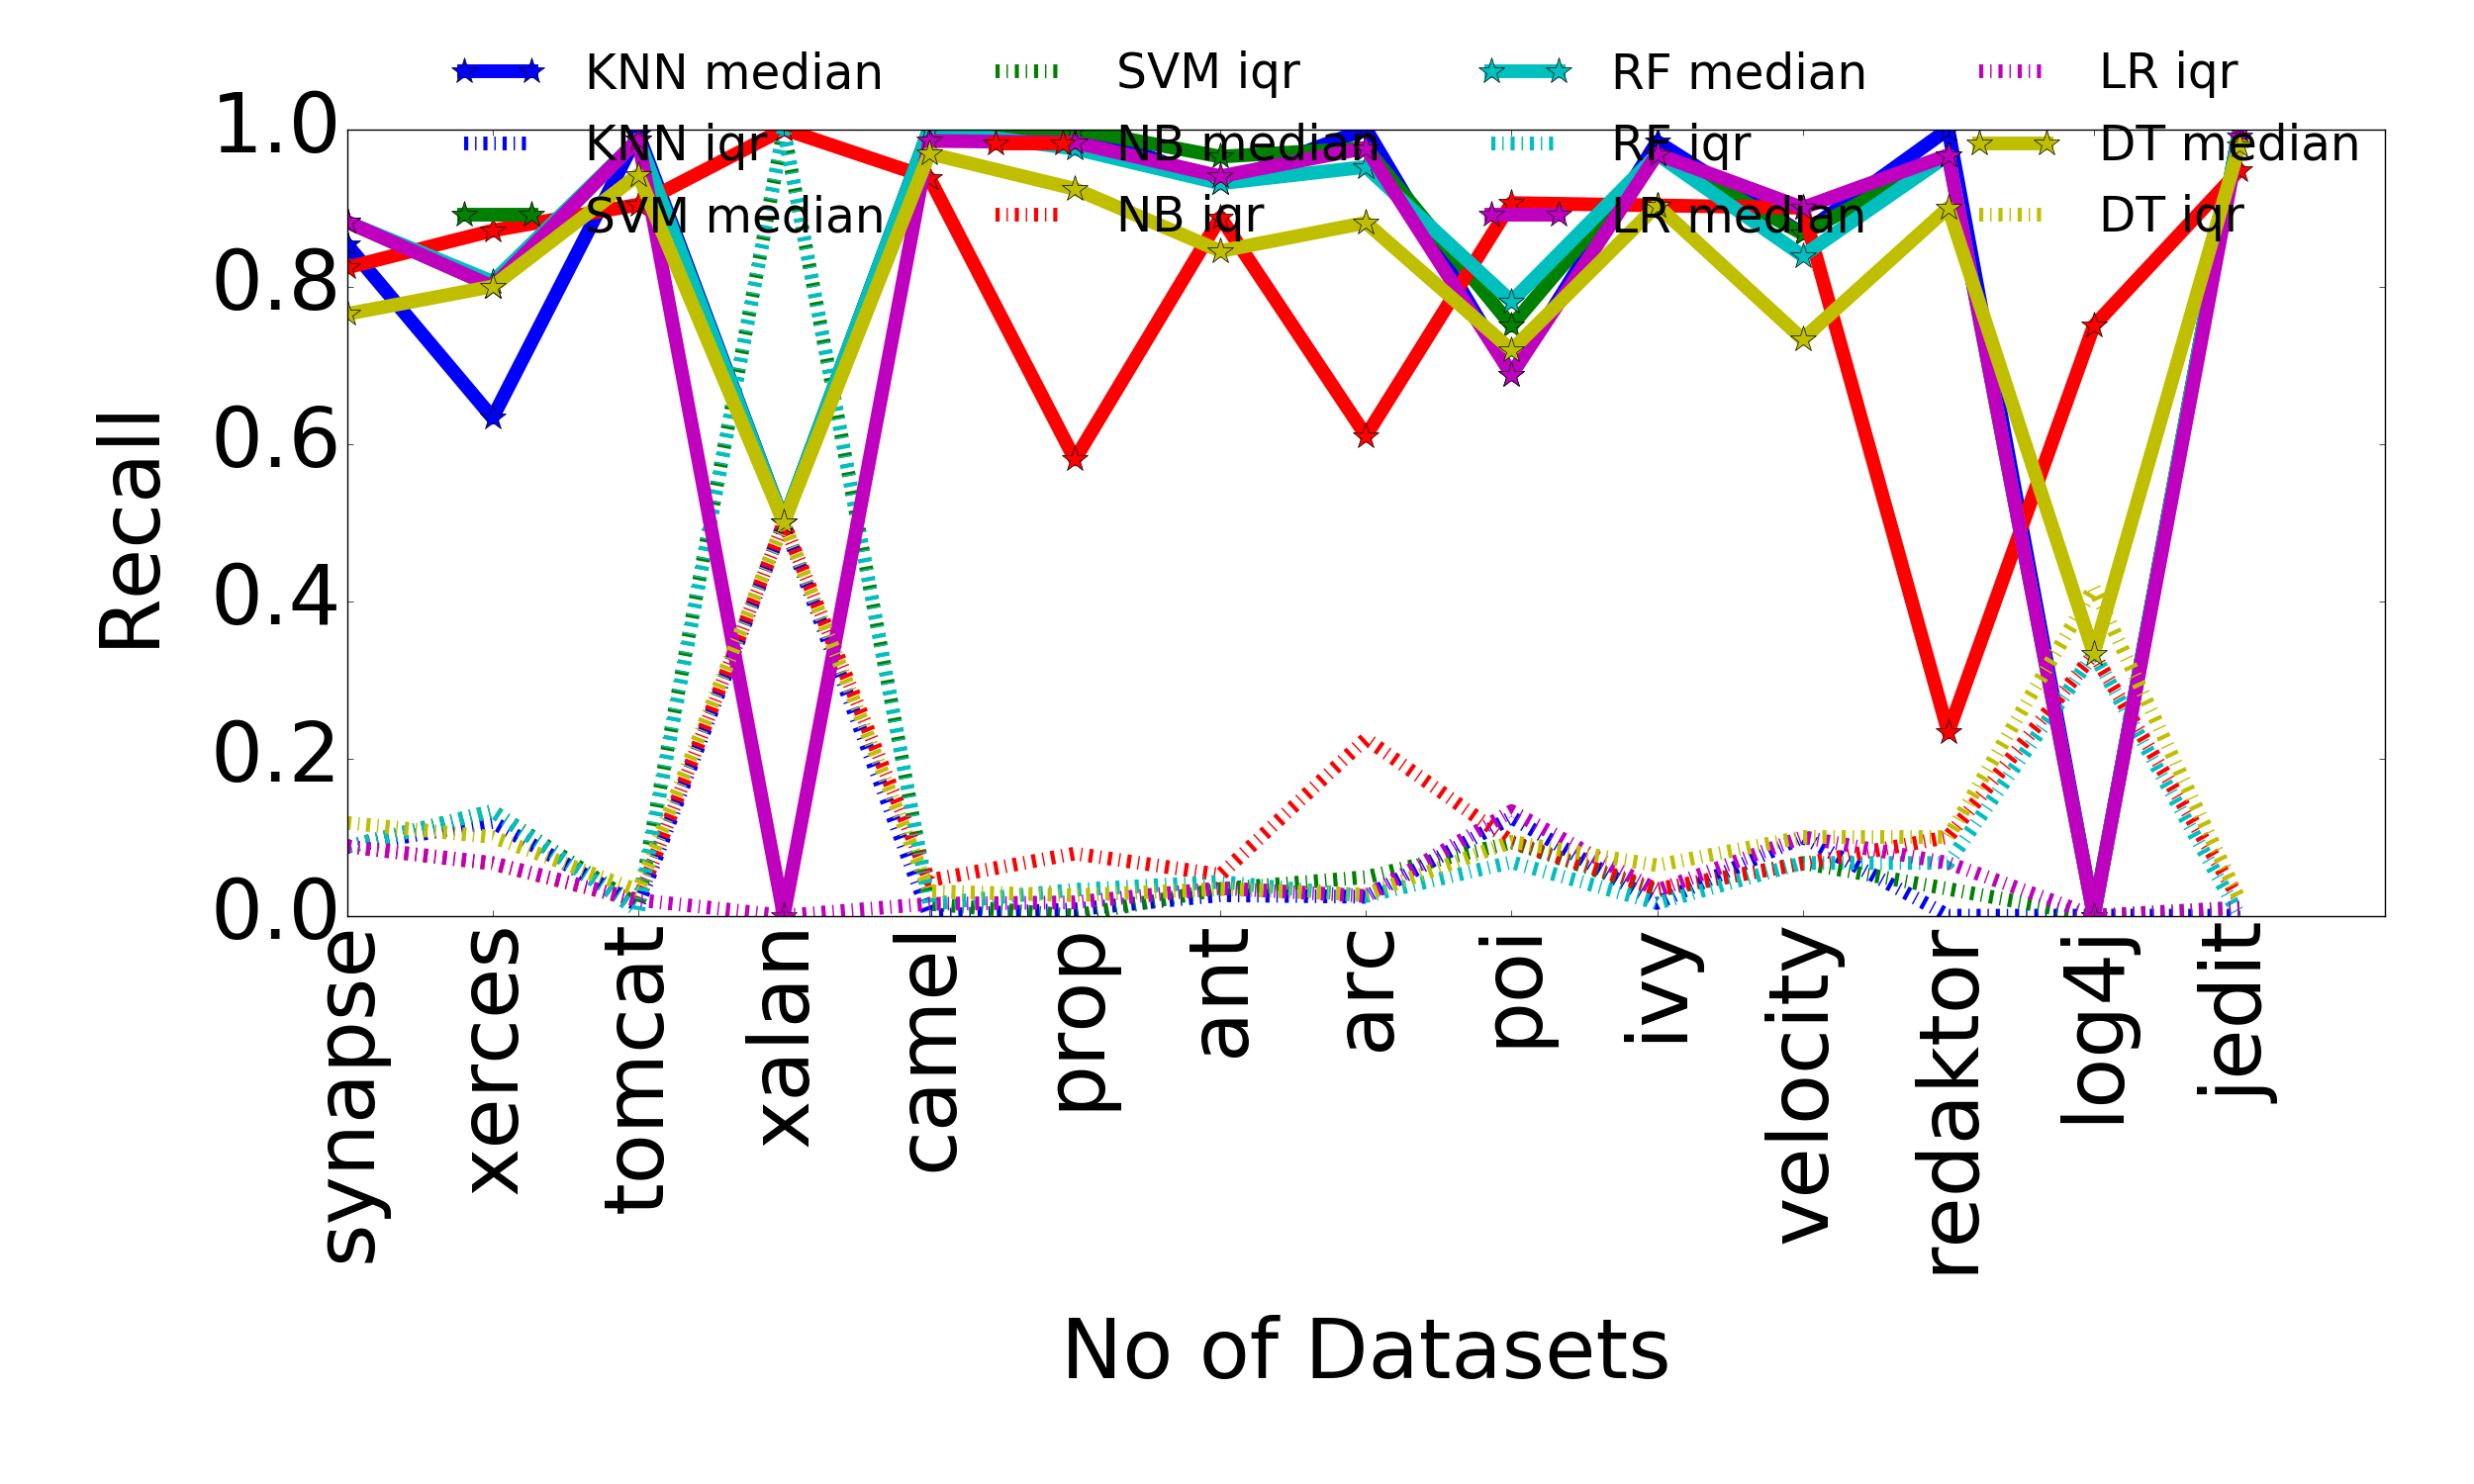
\includegraphics[width=\linewidth]{Recall_nosmote.png}
  {\bf Figure~\ref{fig:nosmote}b:} Recall Without smote.
  \end{center}
    \end{minipage}
    \begin{minipage}[b]{0.49\linewidth}
        \begin{center}
        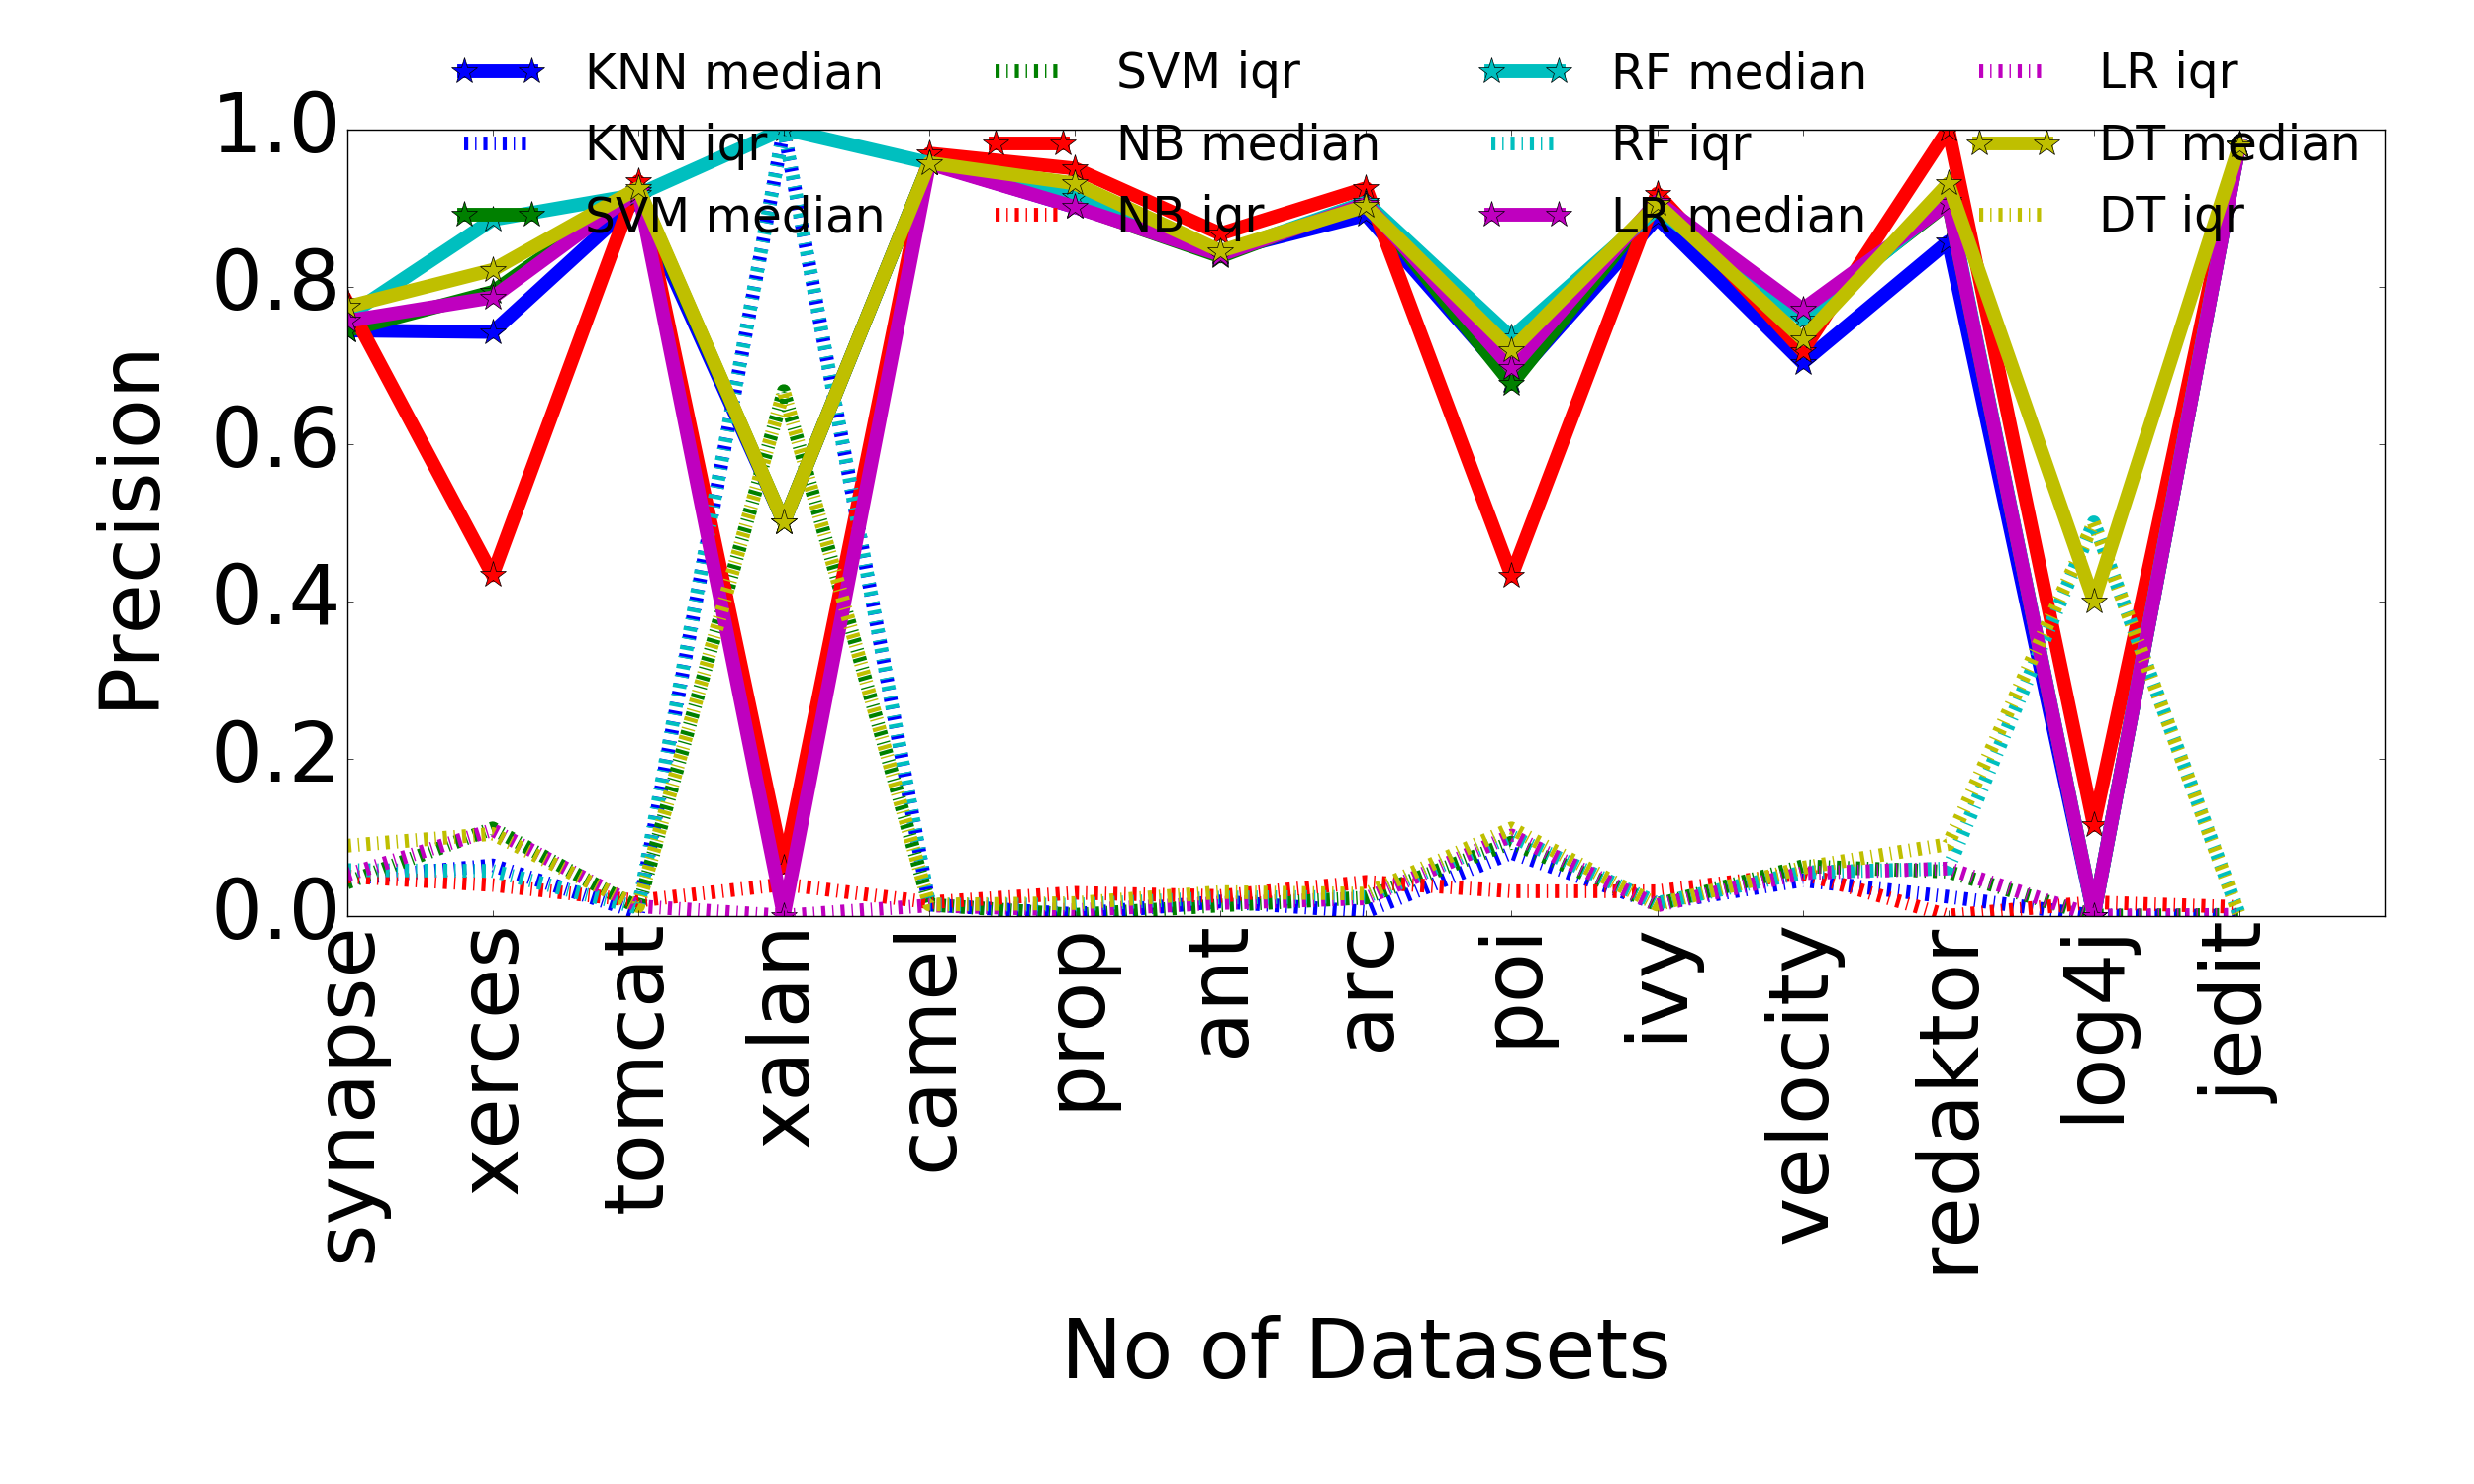
\includegraphics[width=\linewidth]{Precision_nosmote.png}
  {\bf Figure~\ref{fig:nosmote}c:} Precision Without smote.
  \end{center}
    \end{minipage}
    \begin{minipage}[b]{0.49\linewidth}
        \begin{center}
        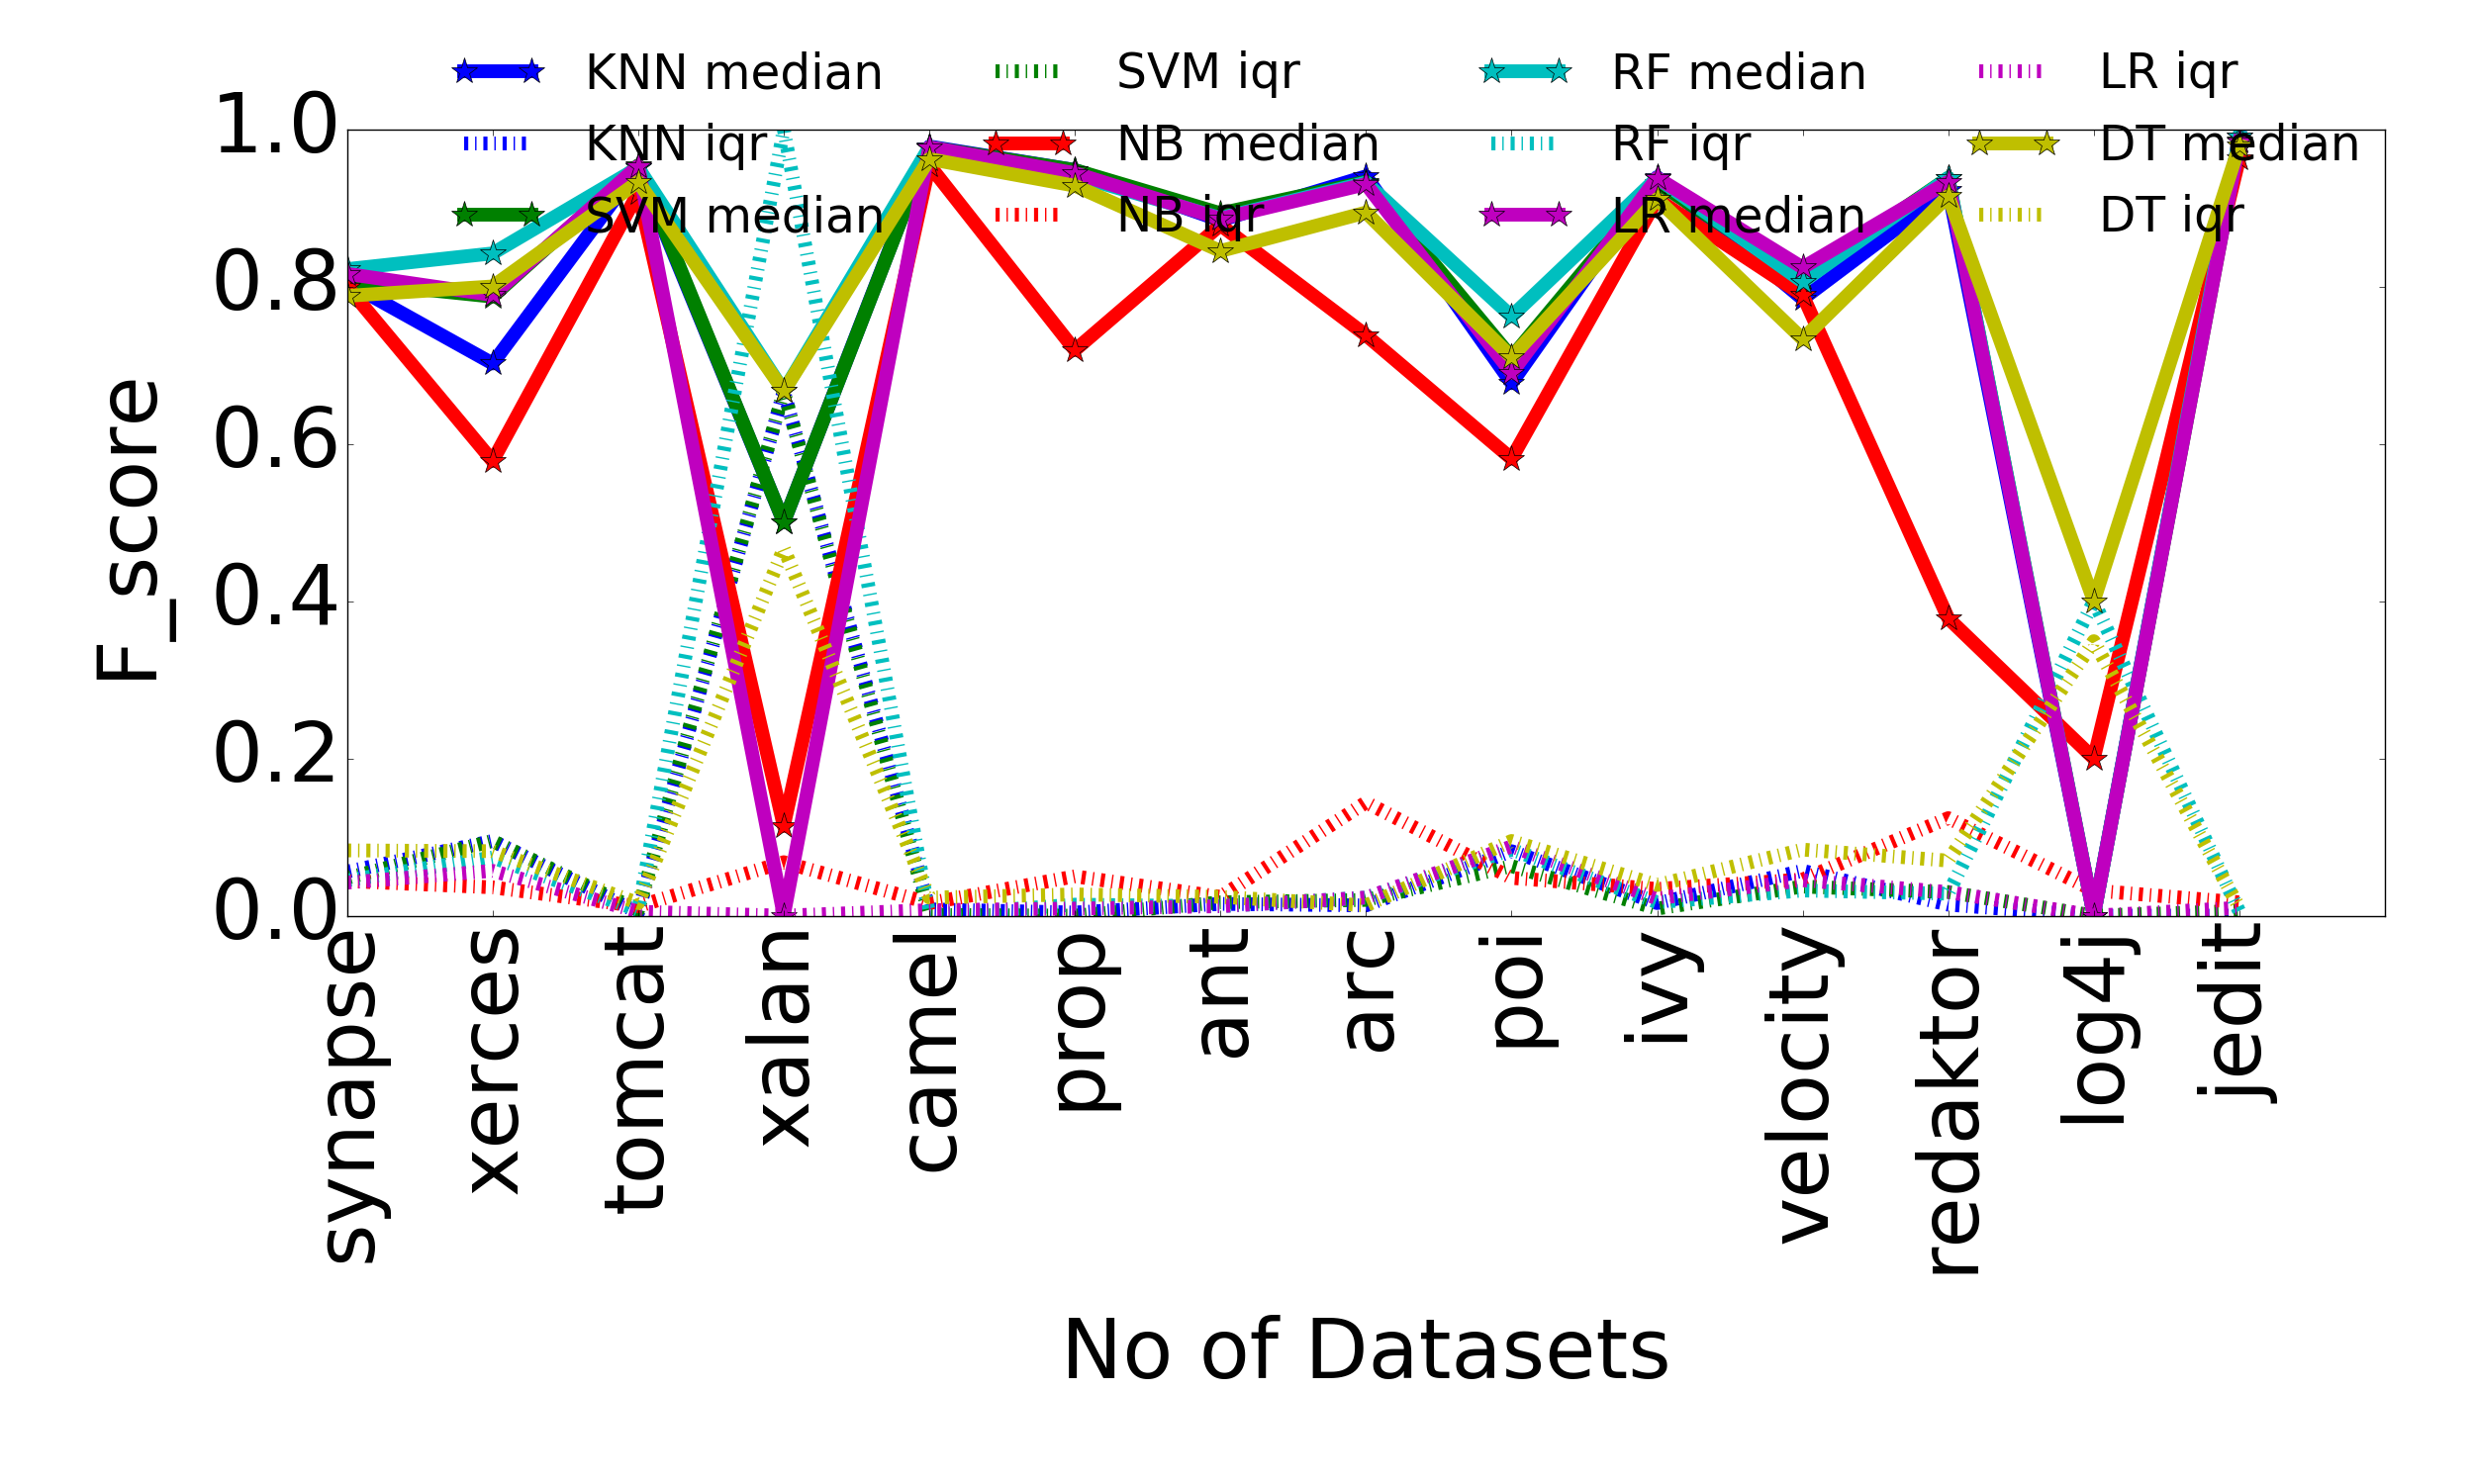
\includegraphics[width=\linewidth]{F_score_nosmote.png}
  {\bf Figure~\ref{fig:nosmote}d:} F1 score Without smote.
  \end{center}
    \end{minipage}
    \caption{Results comparing 6 learners for each measure without smote}\label{fig:nosmote}
\end{figure*}


\begin{figure*}[!htbp]
    \centering
    \begin{minipage}[b]{0.49\linewidth}
        \begin{center}
        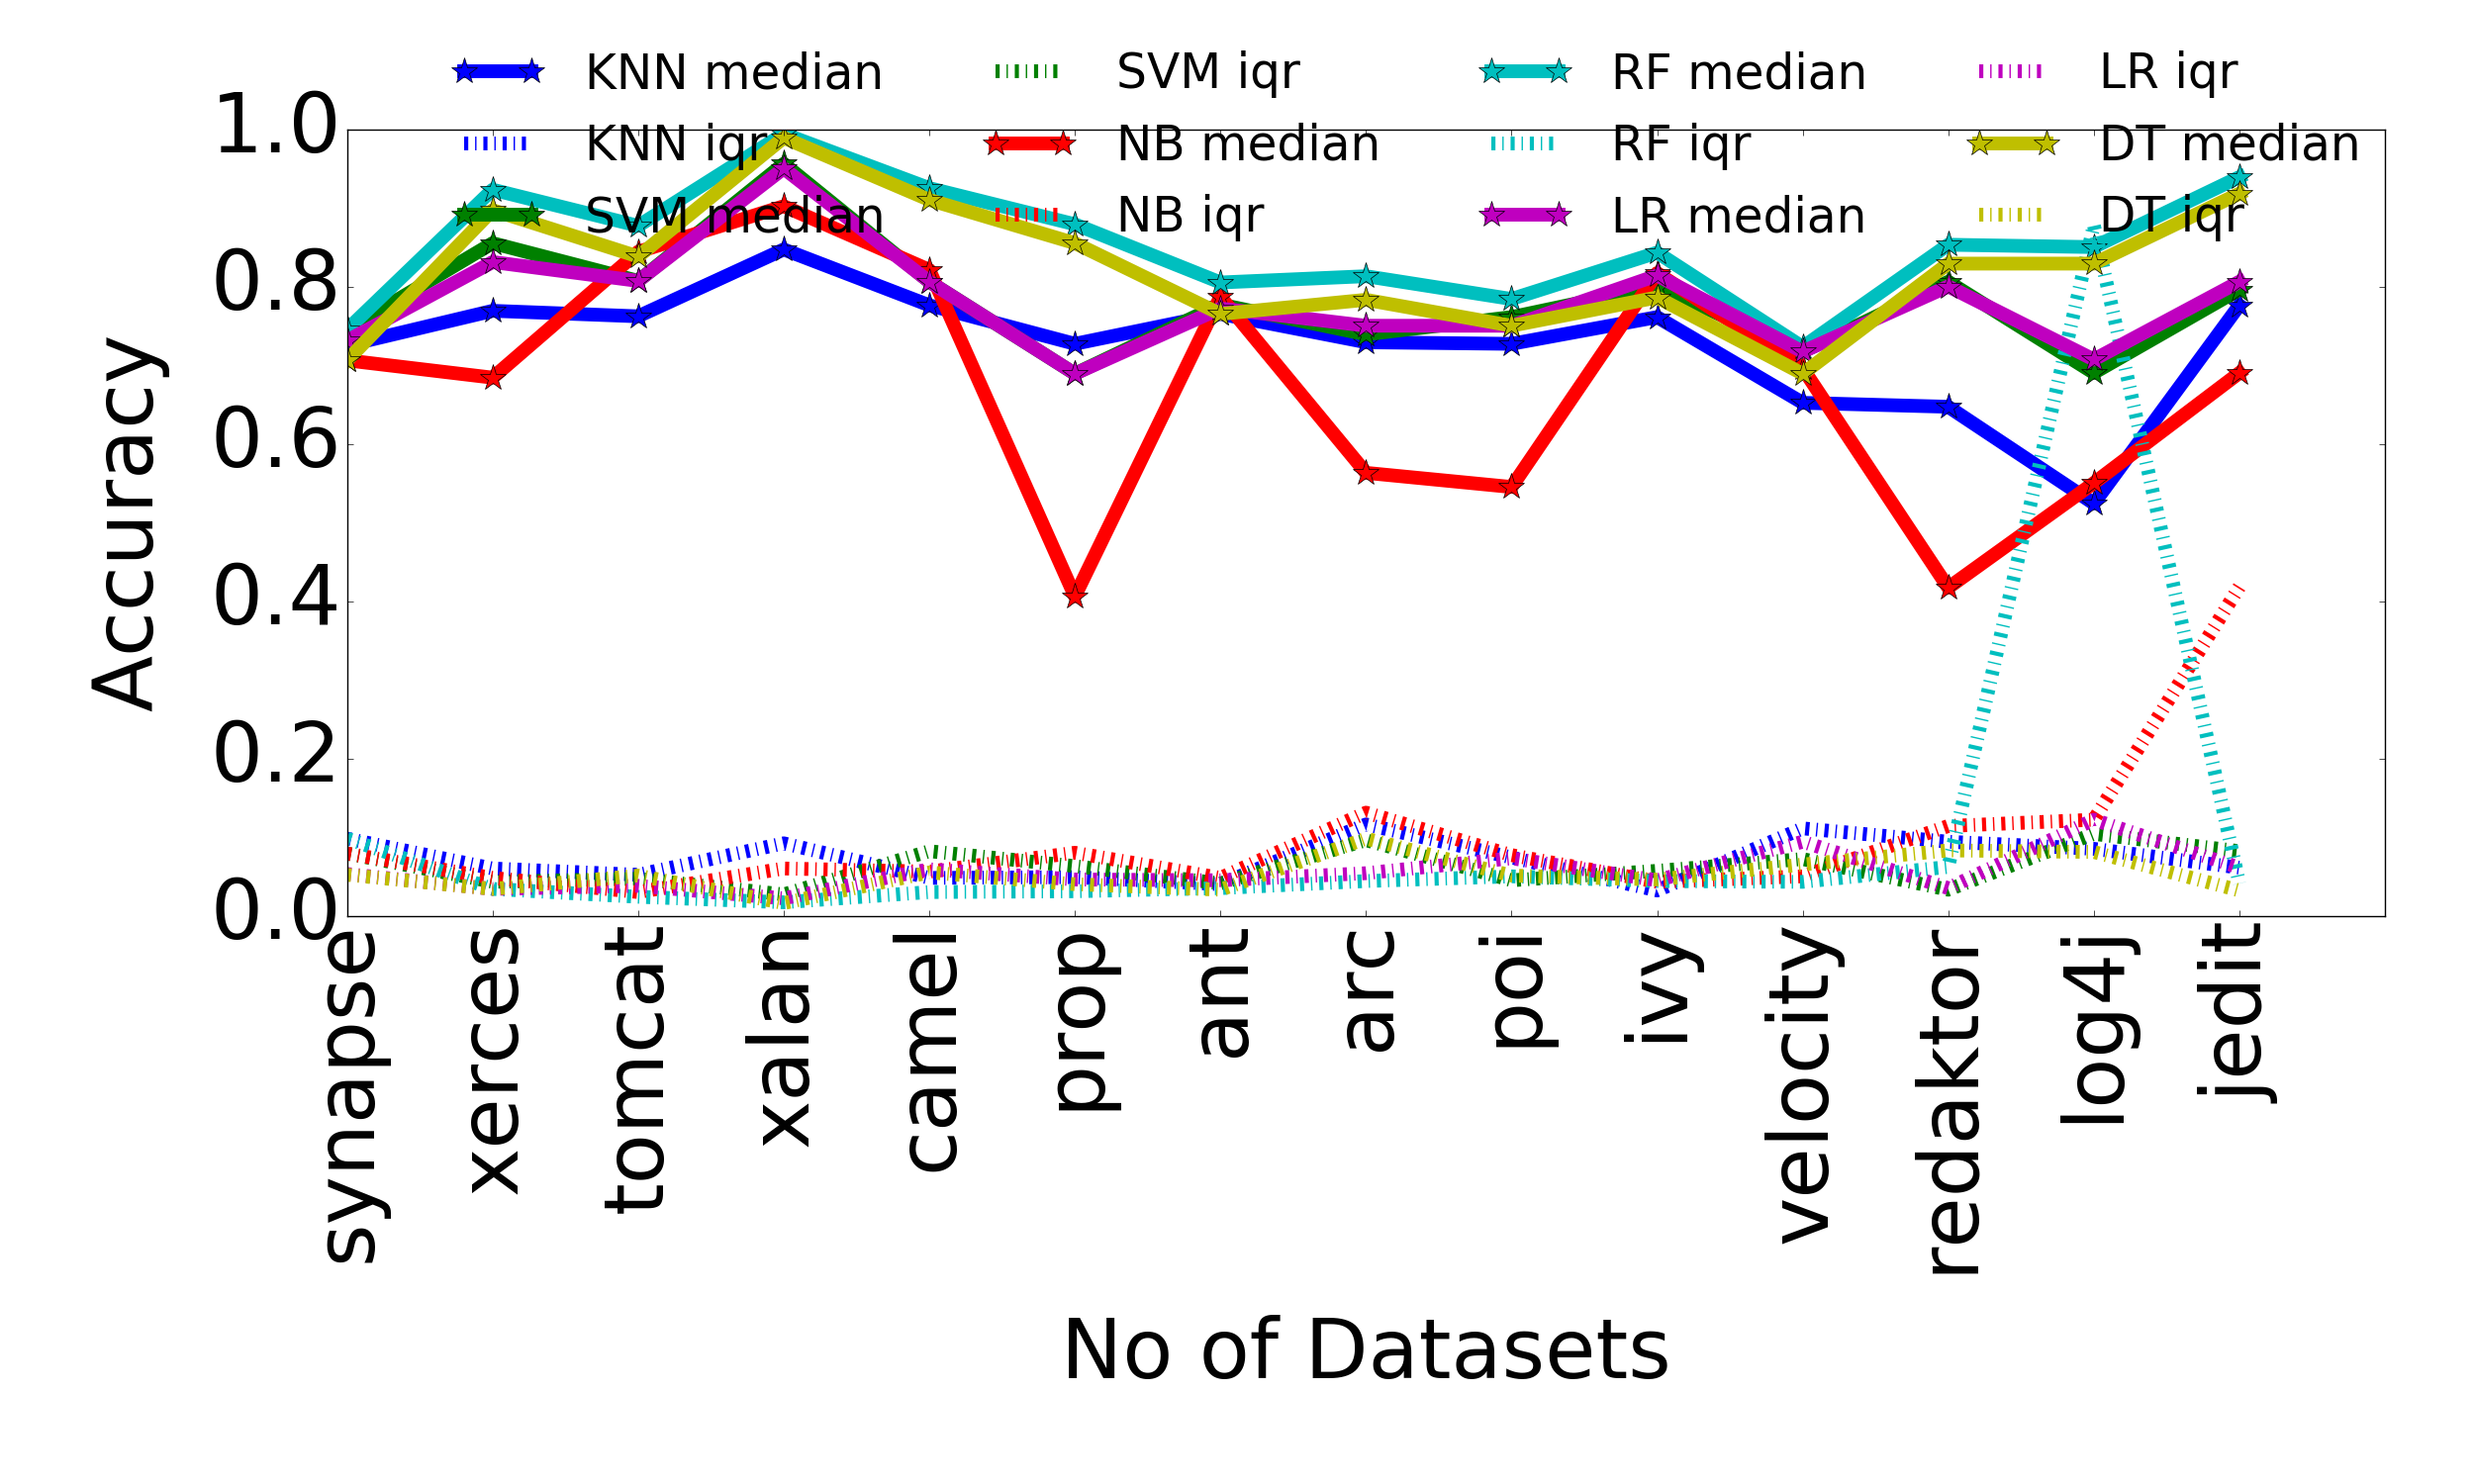
\includegraphics[width=\linewidth]{Accuracy_smote.png}
  {\bf Figure~\ref{fig:smote}a:} Accuracy With smote.
  \end{center}
    \end{minipage}%
    \begin{minipage}[b]{0.49\linewidth}
        \begin{center}
        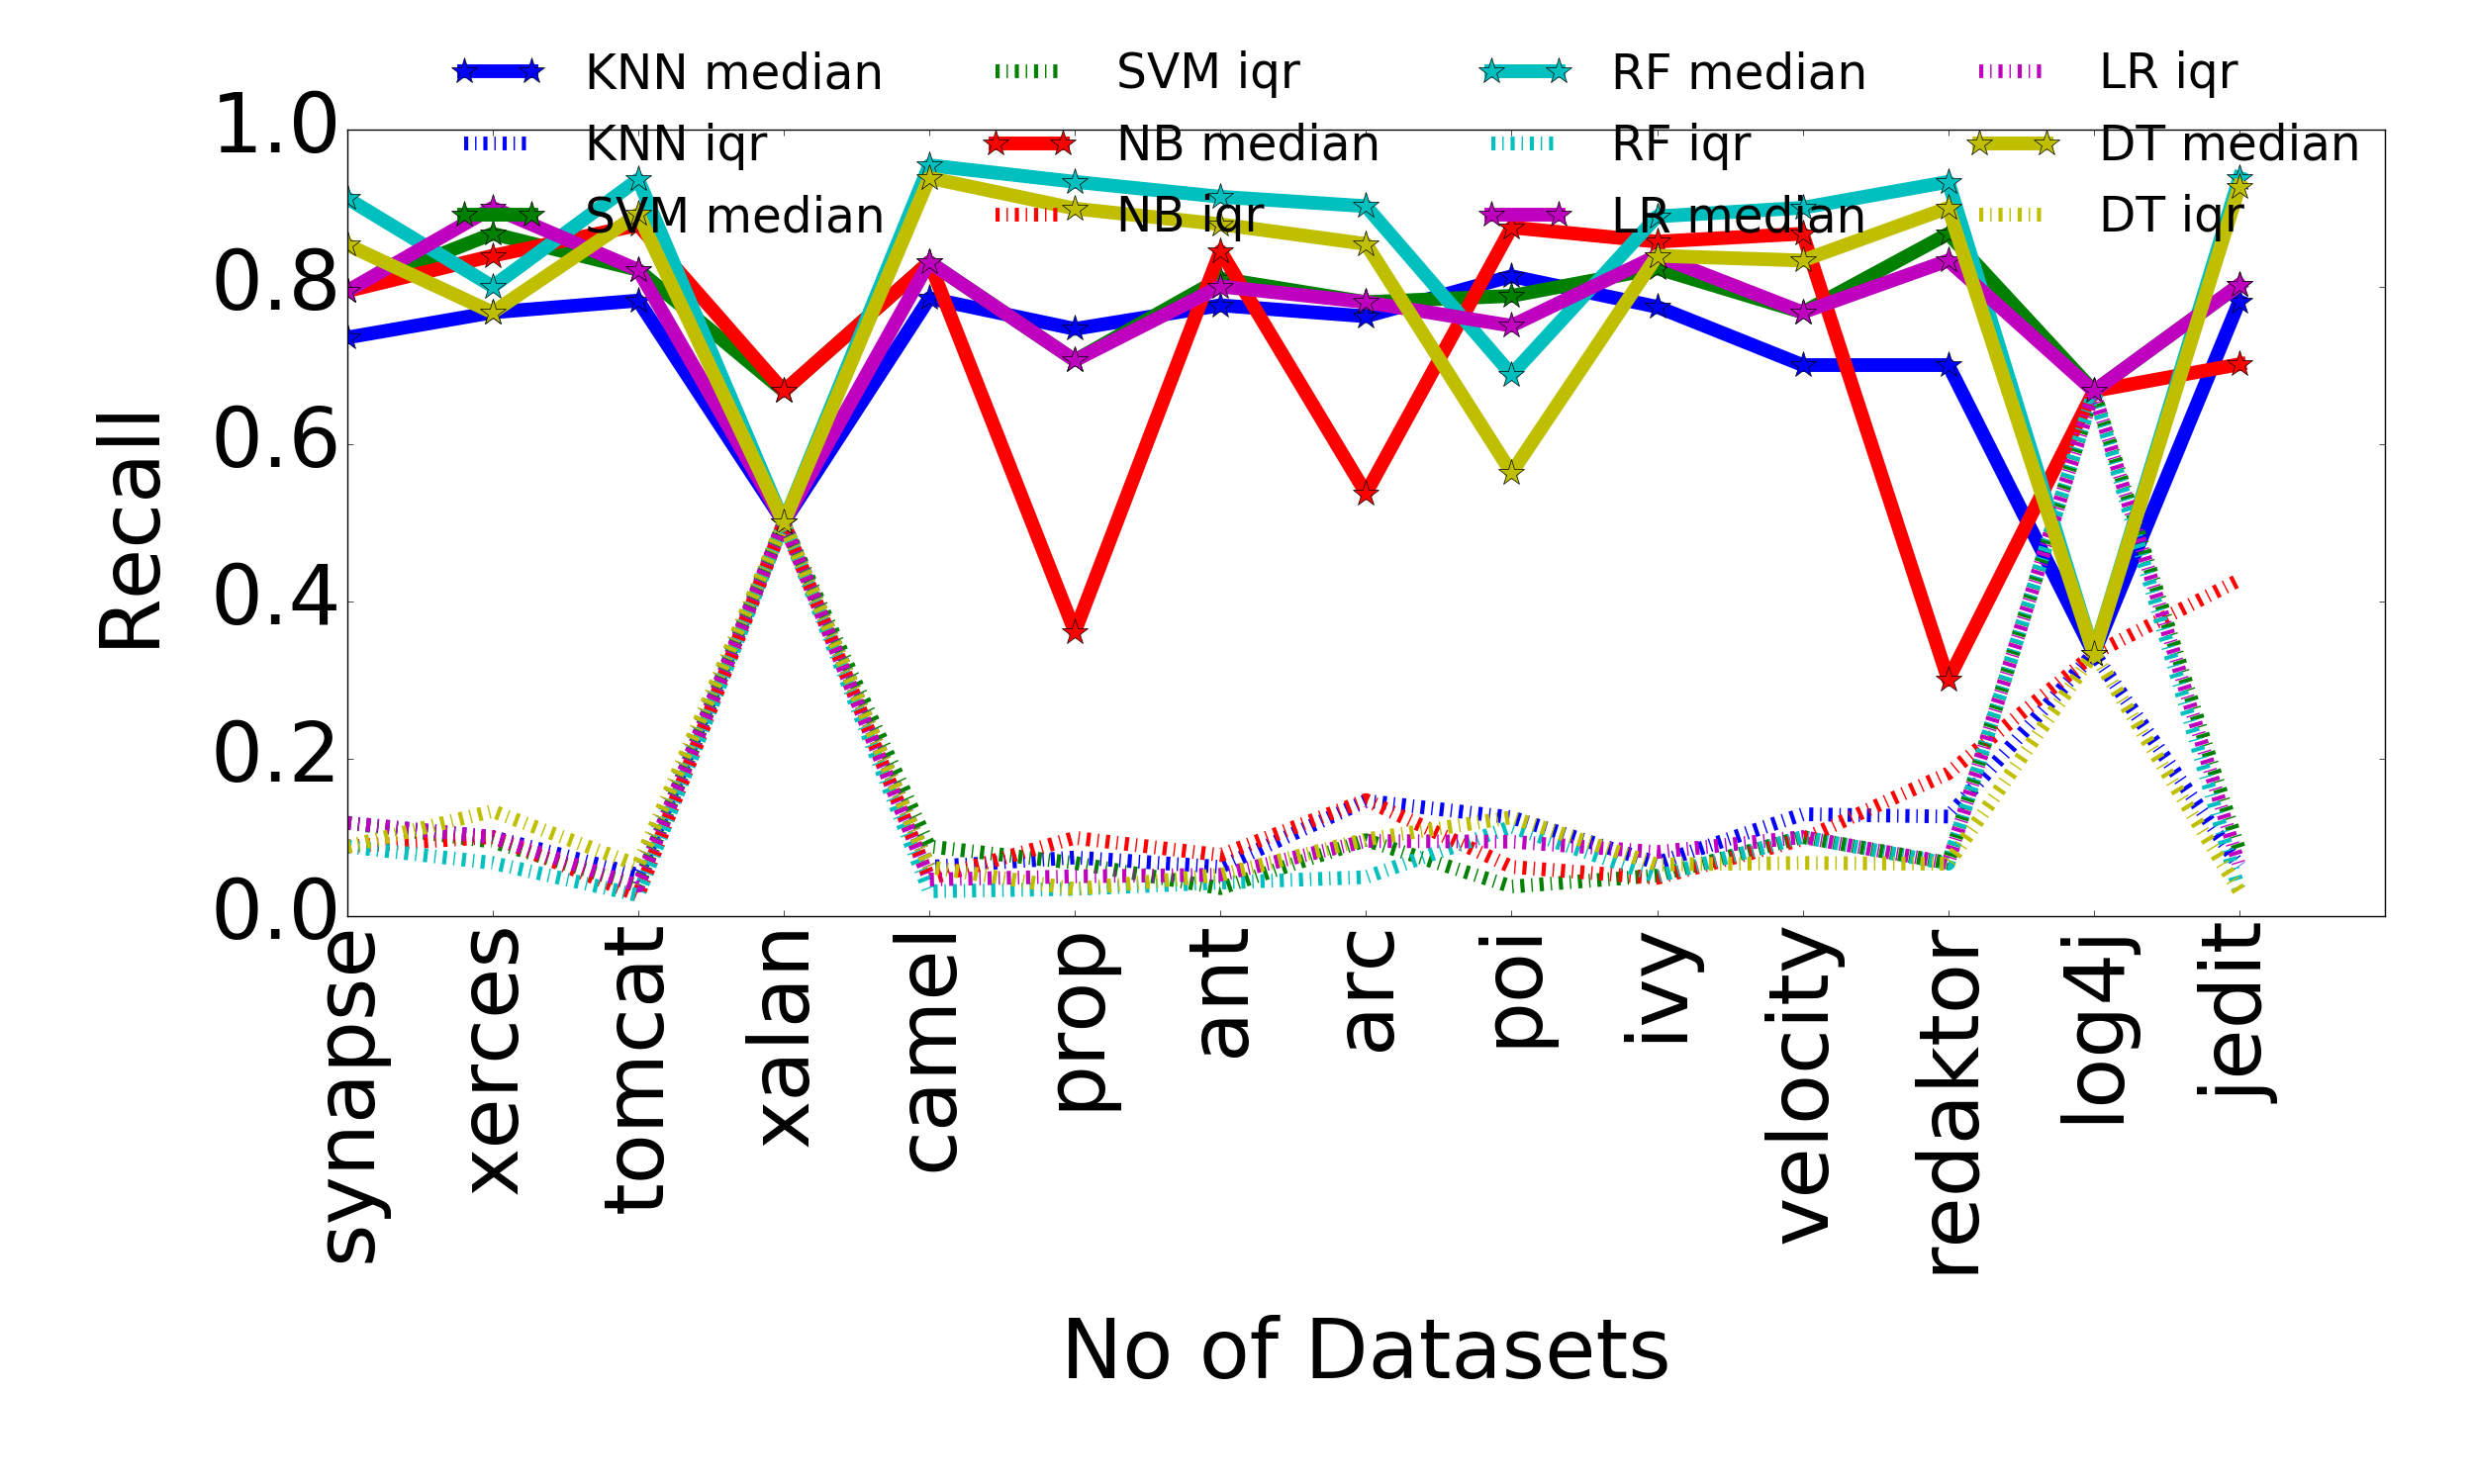
\includegraphics[width=\linewidth]{Recall_smote.png}
  {\bf Figure~\ref{fig:smote}b:} Recall With smote.
  \end{center}
    \end{minipage}
    \begin{minipage}[b]{0.49\linewidth}
        \begin{center}
        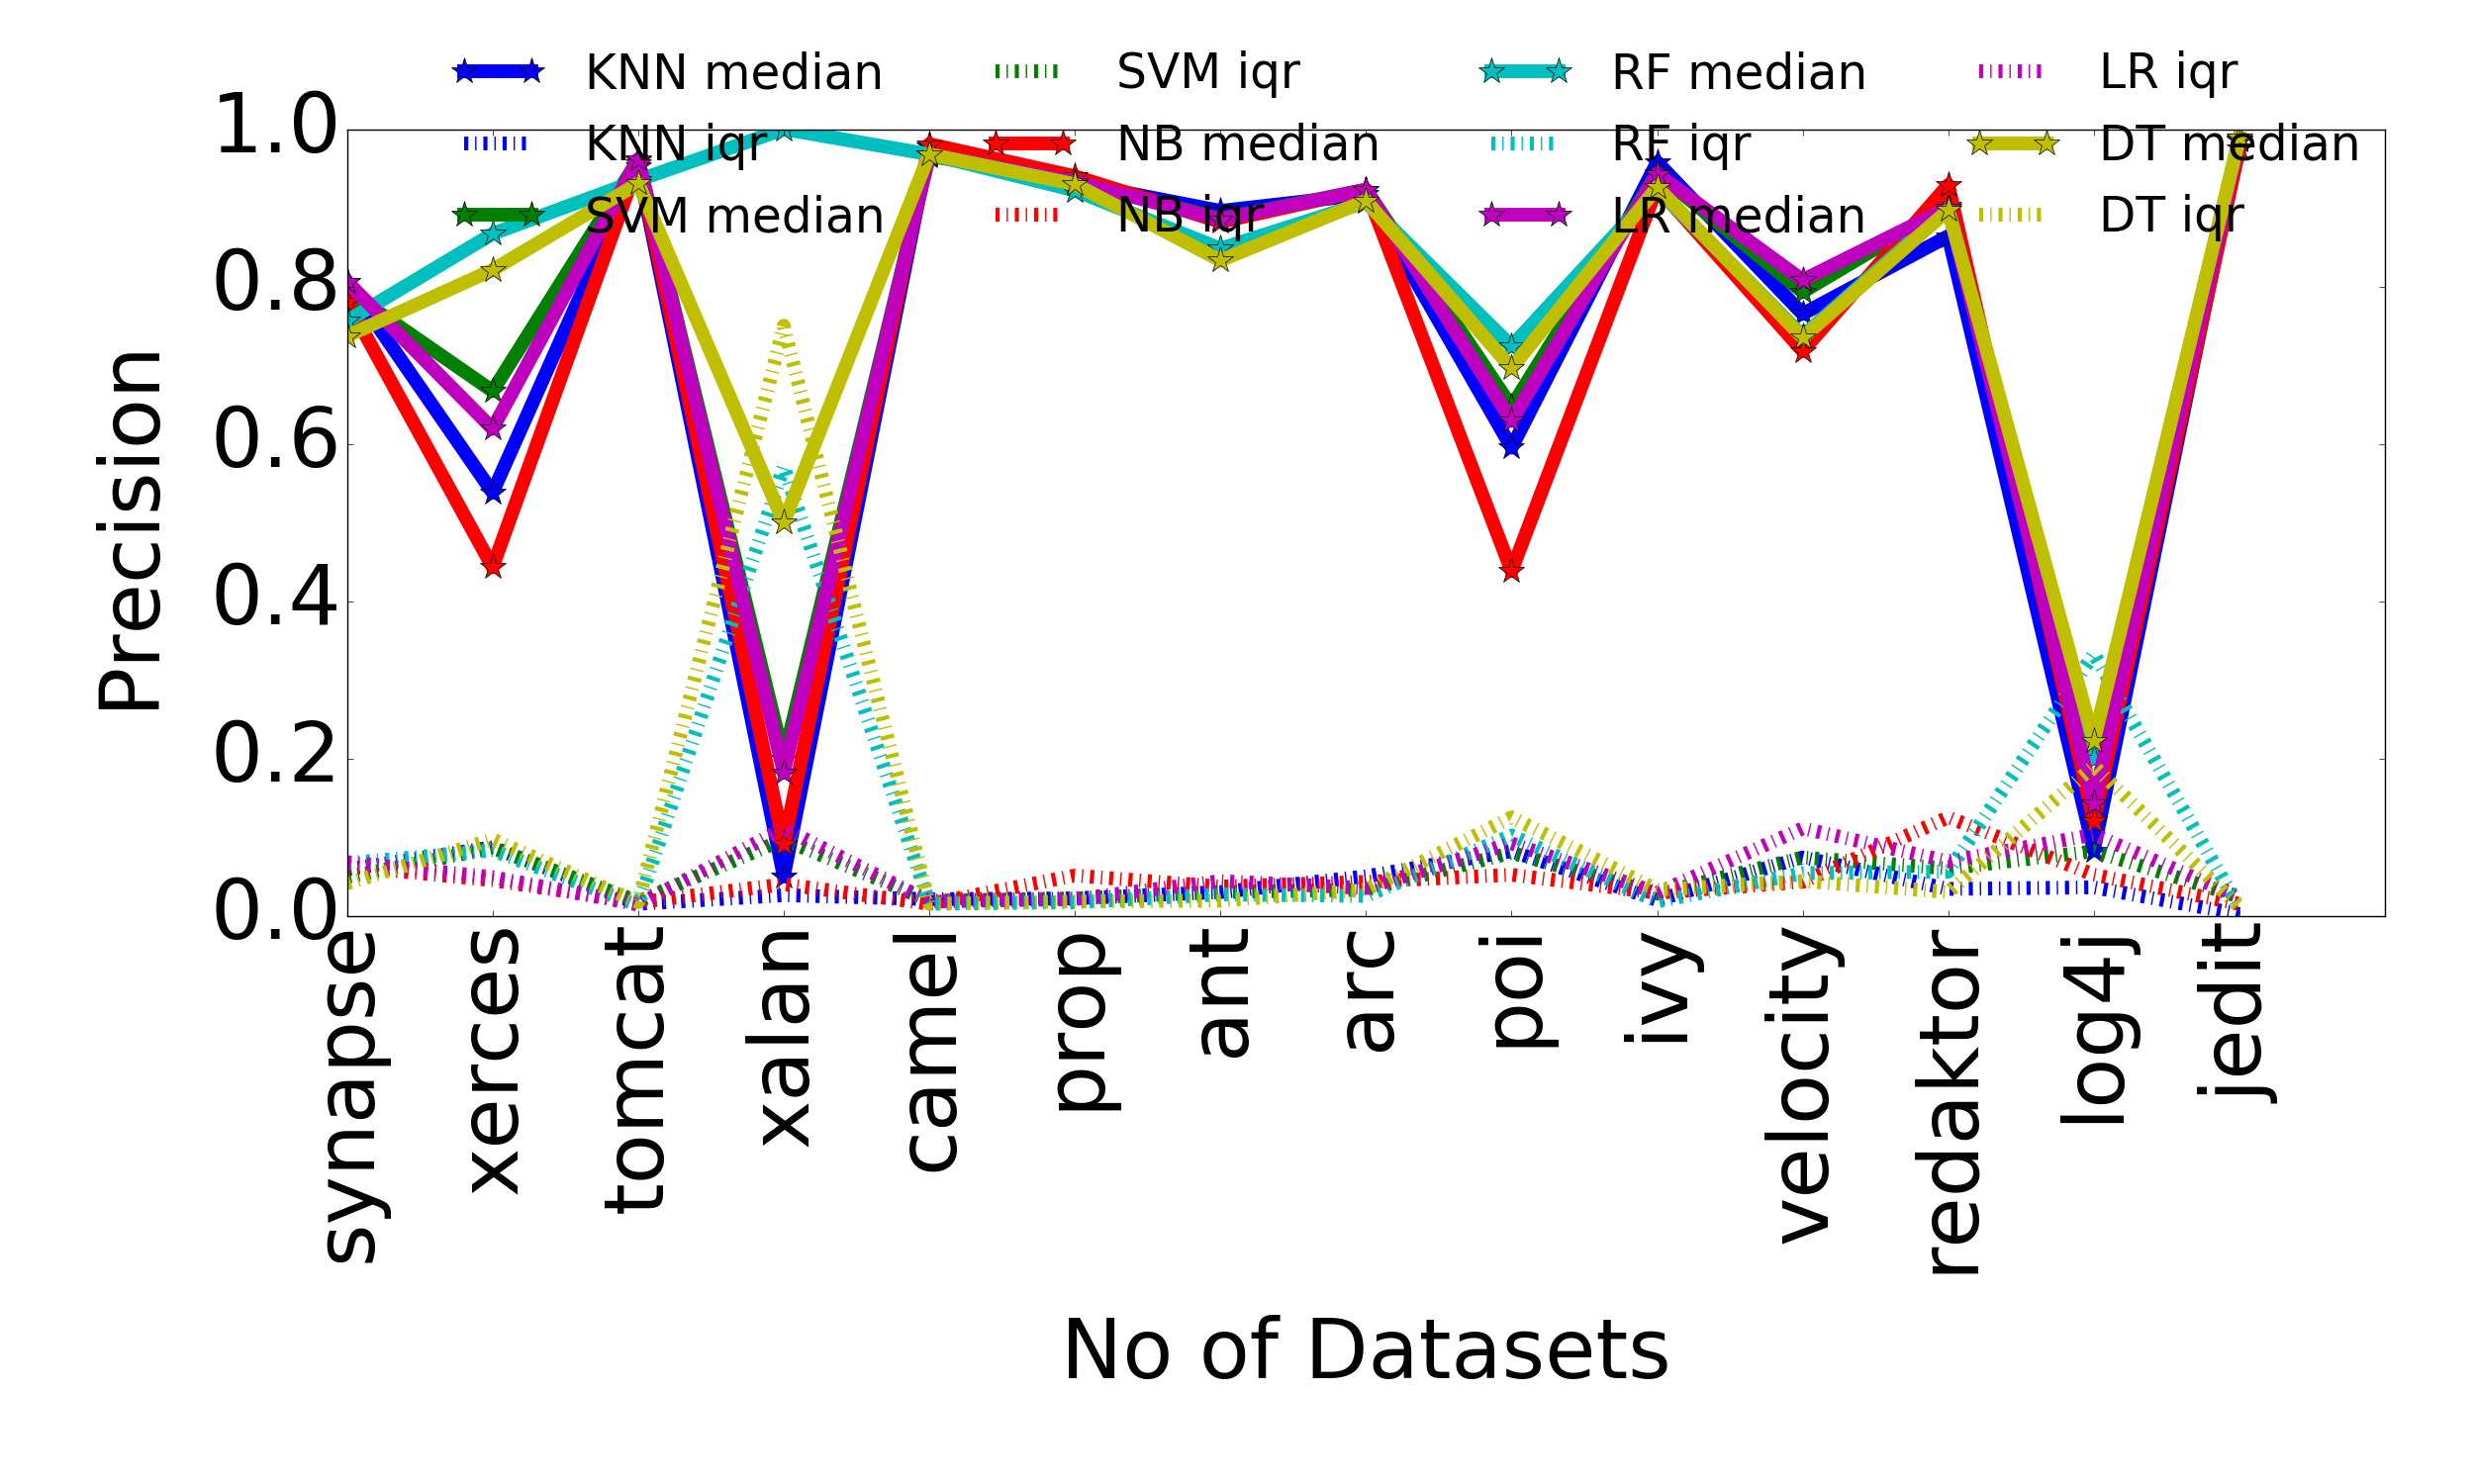
\includegraphics[width=\linewidth]{Precision_smote.png}
  {\bf Figure~\ref{fig:smote}c:} Precision With smote.
  \end{center}
    \end{minipage}
    \begin{minipage}[b]{0.49\linewidth}
        \begin{center}
        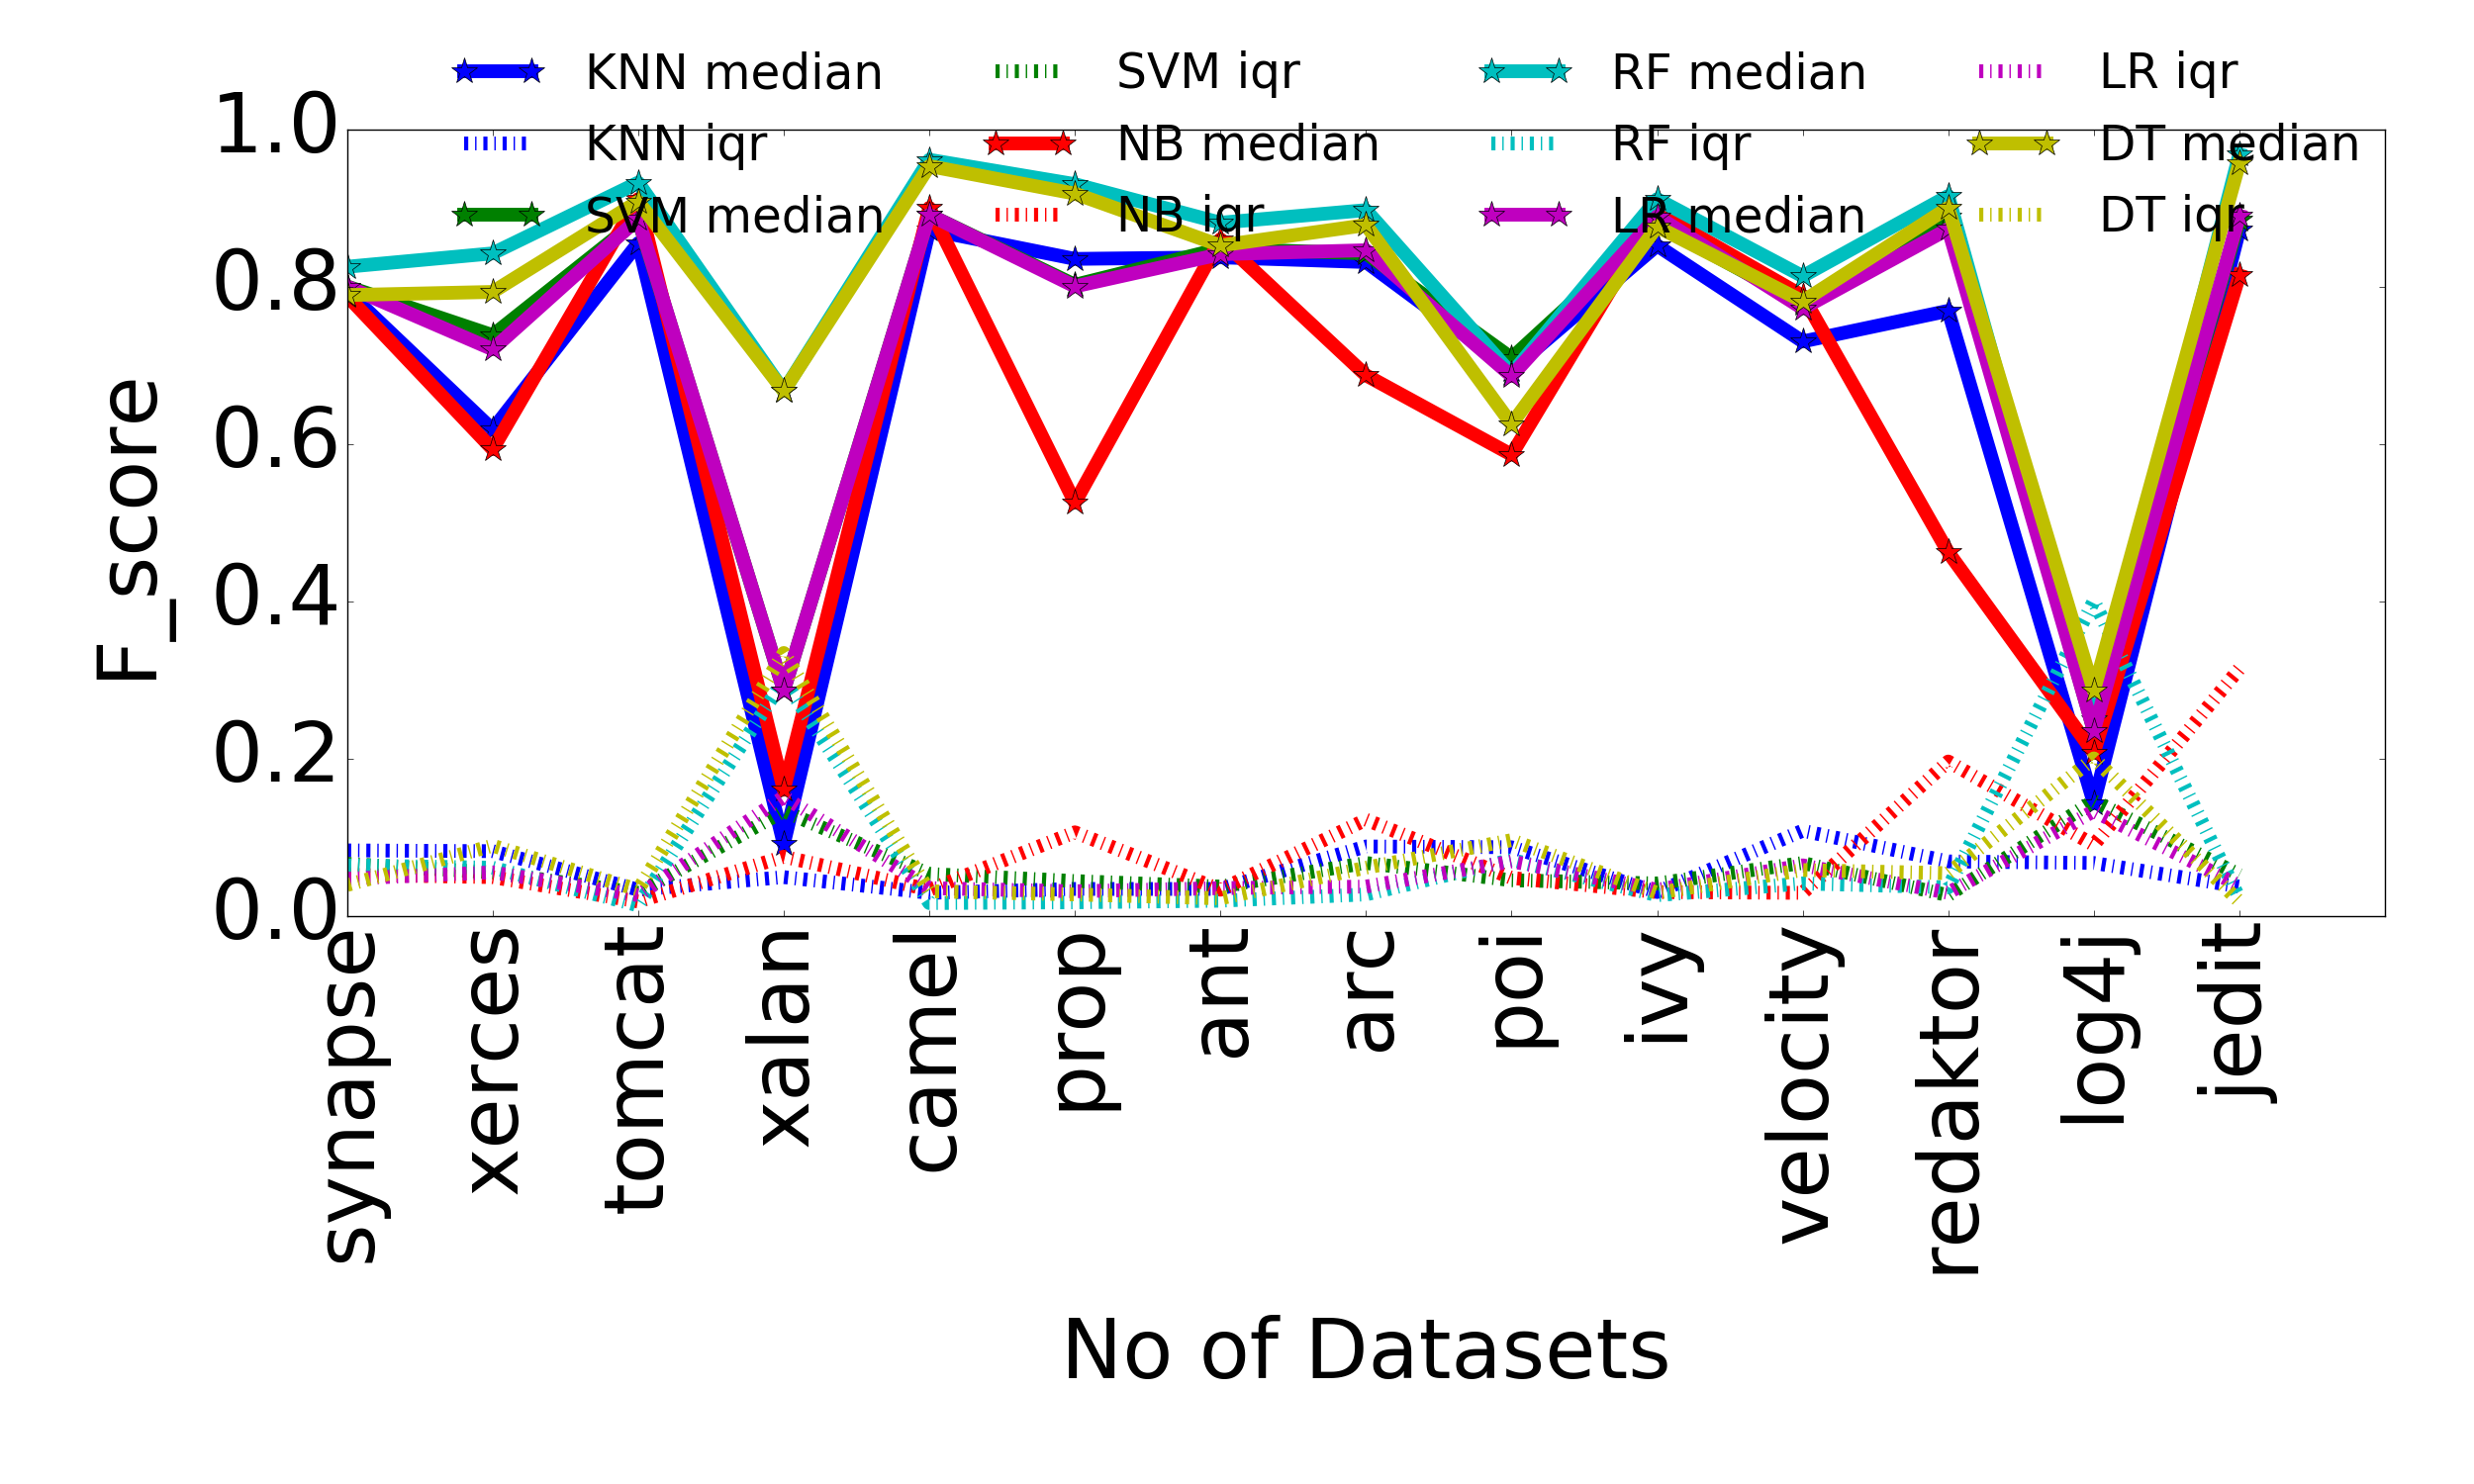
\includegraphics[width=\linewidth]{F_score_smote.png}
  {\bf Figure~\ref{fig:smote}d:} F1 score With smote.
  \end{center}
    \end{minipage}
    \caption{Results comparing 6 learners for each measure with smote}\label{fig:smote}
\end{figure*}


\begin{figure*}[!htbp]
    \centering
    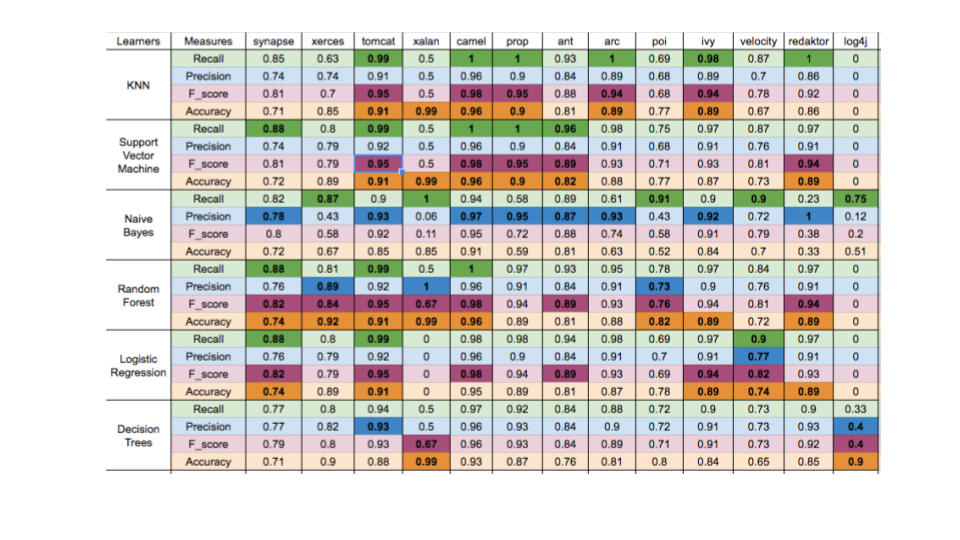
\includegraphics[scale=0.50]{non-smote.png}
        \caption{Without Smote Results}
    \label{fig:tablenosmote}
\end{figure*}

\begin{figure*}[!htbp]
    \centering
    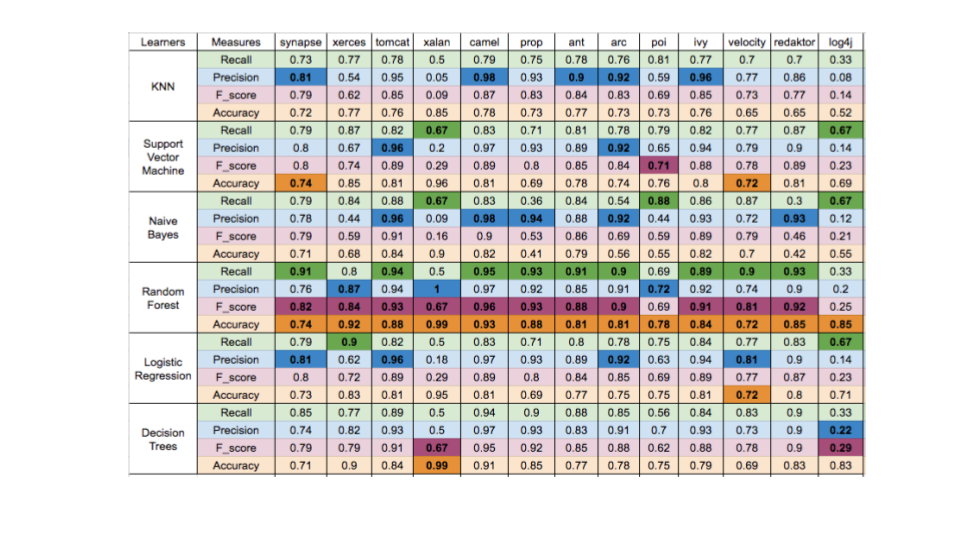
\includegraphics[scale=0.50]{smote.png}
        \caption{Smote Results}
    \label{fig:tablesmote}
\end{figure*}

\subsection{\textbf{The Scott-Knott Test}}

Scott-Knott Effect Size Difference
(ESD) test is an enhancement of the standard Scott-Knott
test (which cluster distributions into statistically
distinct ranks~\cite{scott1974cluster}), which makes no assumptions about the underlying distribution and takes the effect size into
consideration~\cite{tantithamthavorn2015empirical}. After the predicted values are computed, we pass the accumulated values to a Scott-Knott Test which compares 6 learners for each of these measures F-Score, Recall, Accuracy, Precision and False Alarm. The results are available to user by helper methods.

\subsection{\textbf{The visualizations}}

We have included a visualization script, when executed with a pickle file displays the pretty visualization of all the learners. Currently this is not implemented as a part of output. A user has to dump the results in a pickle file and run the script manually.

\section{Results}
\label{results}
 Figures~\ref{fig:nosmote} and ~\ref{fig:smote} represents all the datasets without performing smote and with smote respectively. 4 different graph represents each evaluation measure. X-axis represents all the 14 datasets and y-axis represents scores. Each splod line represents median value for 6 learners and dashed line represents variance of 25 numbers (ie, 75th percentile - 25th percentile). From the graphs we can see how stable our results are since variance is less than 10\%.
 
 Now to see exact difference between smote and without smote, see figures~\ref{fig:tablenosmote} and ~\ref{fig:tablesmote}. These figures show each learners all evaluation scores and column represents each dataset median values. Now to read these figures take any colum, and select 1 evaluation measure and follow its background color in the same column. The bold mark for such color represents which learner preforms the best. From figure~\ref{fig:tablenosmote}, we observed that Logistic regression, random forest and nearest neighbor has almost equal proportions of winners among different datasets which was the expected results from our baseline paper~\cite{ghotra2015revisiting}. 
 
 But we found astonishing results while reading the numbers from figure~\ref{fig:tablesmote} which is with smote. We observed that for recall, f1 score and accuracy, Random forest performed the best. Also, we got less variance in smote results than the non-smote.

The run times for most of the data sets except 2 data sets Tomcat and Xalan took close to 20 minutes. For Tomcat and Xalan it took close to 2 hours. The package was deployed on HPC machines.

\section{Conclusion}
\label{conclusion}

We were able to reproduce the baseline paper "Revisiting the impact of classification techniques on the performance of defect prediction models" with the same conclusions what ghotra et al. found which are results without smote. But after applying smote, Random Forest outperformed every other learner. To control the high variance and most data sets have minority defective class, we highly recommend to use smoting. Comparing the run times and performance, we suggest to use Random Forest if the data sets are not big as it has larger runtime overhead.

\section{Future Work}
\label{future}
In future, we can improve this pip package once other users start reporting issues. Additional features can be added such as:
\begin{itemize}
 \item We can think of implementing cross project defect prediction.
 \item We can have binary classification, as well as to predict quantities of defects which is regression based model.
 \item The algorithm for smoting is hard-coded to "ball tree", this can be parametrized.
 \item The Split criteria and K value in K Nearest Neighbours are hard-coded, these can be parametrized.
 \item The learners currently doesn't support any tuning, which can implemented.
 \item Pretty visualizations can be added.
\end{itemize}

\balance

\bibliographystyle{abbrv}
\medskip
\bibliography{ref}

\end{document}